\documentclass[11pt]{article}
\usepackage[cm]{fullpage}
\usepackage{fancyvrb}
\usepackage[superscript,biblabel]{cite}
\usepackage[acronyms]{glossaries}
\bibliographystyle{plain}
\usepackage{url,hyperref}
\hypersetup{
   citecolor=black,
   colorlinks=true,
   linkcolor=blue,
   filecolor=magenta,
   urlcolor=blue,
}
\usepackage{csquotes}
\usepackage{makeidx}

\usepackage{float}
\usepackage{graphicx}
\usepackage{amssymb}
\usepackage{amsmath}
\usepackage{pifont}% http://ctan.org/pkg/pifont
\newcommand{\cmark}{\ding{51}}%
\newcommand{\xmark}{\ding{55}}%
%% \usepackage{tabularx}
\usepackage{caption}

\makeglossaries
\longnewglossaryentry{acma}{ name ={{ACMA}}}
{
The Australia Communications and Media Agency. 
\href{https://www.acma.gov.au/amateur-radio}{ACMA Link}
\par
Callsign policy is located here: \href{https://www.acma.gov.au/sites/default/files/2024-05/Amateur\%20radio\%20call\%20sign\%20policy\_April\%202024.pdf}{Callsign Policy at ACMA}
}

\longnewglossaryentry{vna}{ name ={{VNA}}}
{
A Vector Network Analyzer (VNA) is a device that measures the power and characteristics of a high-speed signal, such as amplitude and phase, going into and out of a component or network. It can be used to measure the impedance of an antenna, which allows you to design a matching circuit to optimize the antenna's electrical match to its feed. 
}

\longnewglossaryentry{qrv}{ name={{QRV}} }
{
To begin operation with at least one station on the air
actively taking CQ requests and logging.
}


\longnewglossaryentry{hf} { name={{HF}} }
{
High frequency for amateur bands ranges that apply to the expedition
are between 160 meters through 6 meters.  The Australian amateur
radio license will not permit operation on 60 meters.}

\longnewglossaryentry{iota} { name={{IOTA}} }
{Islands on the Air. 
Established in 1964, it promotes radio contacts with stations located on islands around the world to enrich the experience of all active on the amateur bands and, to do this, it draws on the widespread mystique surrounding islands.}


\longnewglossaryentry{rsgb} { name={{RSGB}} }
{
The Radio Society of Great Britain (RSGB) is the United Kingdom's recognized national society for amateur radio operators. The society was founded in 1913 as the London Wireless Club, making it one of the oldest organizations of its kind in the world.
}


\longnewglossaryentry{lhi} { name={{LHI}} }
{
Lord Howe Island.
}


\longnewglossaryentry{crankir} { name={{CrankIR}} }
{
The Crank-IR is a vertical antenna made by SteppIR.
\par
The SteppIR CrankIR is a portable Ham radio antenna that can be used for park activations. It has a standard model that can be used for 6M through 40M, and it also has an optional tunable Radial Unit. The antenna is lightweight, high performance, and extremely portable. It has a patented folded design that allows for a 40\% reduction in size with only a 0.3dB reduction in performance compared to a full length vertical.
}

\longnewglossaryentry{multisingle} { name={{M/S}} }
{
Multi-single (M/S) refers to an operational condition where multiple
operators are using a single radio.
}


\longnewglossaryentry{singletwo} { name={{SO2R}} }
{
Single Operator, Two Radios.  In this scenario a single operator
uses two radios, simultaneously.
}

\longnewglossaryentry{flyin} { name={{Fly-In}} }
{
A reference to a DX'pedition where the team can use commercial
or chartered aircraft to land on the site for operation.  No marine
vessels are required.  A beach-landing on an island by Zodiac or other
water-craft is NOT fly-in.   A helicopter lift operation from a deck
of a sea trawler is NOT fly-in.   
\par
Fly-in DX'peditions are noted to be a bit easier because except for
terrestrial travel from the airport to the operation site the bulk of the
travel was by commercial or chartered aircraft.
}

\longnewglossaryentry{beam} { name={{Beam}} }
{ 
An antenna configuration where the main criteria is that the front to back
gain ratio is pronounced.  A vertical typically does not have this 
condition unless it is part of an array.  See VDA.
}

\longnewglossaryentry{lotw} { name={{LoTW}} }
{
Log Book of the World.  A free service provided by the ARRL
to let amateur radio operators log contacts and receive
confirmation for the QSO.  Contacts collected and verified
in the LoTW system are automatically eligible for credit
for seeking ARRL contest awards, such as DXCC.
}

\longnewglossaryentry{qsl} { name={{QSL}} }
{
Confirmation of the QSO either via electronic means
or more classically by paper cards with the pertinent
information that is required by the officially sanctioned
card-checker system.  For example, ARRL DXCC card checkers
are volunteers who check the authenticity of the QSL records
and help file the paperwork with the ARRL to grant credit
for those QSO as applicable.  QSL'ing is itself an important
part of the DX'pedition.  Amateurs want confirmation either
in LoTW form or QSL card.}

\longnewglossaryentry{eme} { name={{EME}} }
{
Moon-bounce contact.  Otherwise known as Earth-Moon-Earth.  A
highly coordinated method of sending and receiving messages
over usually higher frequencies (like 6 meters) where the moon
itself reflects the signal back to earth.
}

\longnewglossaryentry{wsjtx} { name={{WSJT-X}} }
{WSJT-X is a software package that is used to code and decode 
digital modes in amateur radio.  It is a popular software program
that has facilitated FT-8 mode throughout amateur radio use for the 
past several years.   A common add-on to WSJT-X is JT-Alert.
\par
For most DX operations, the DX station will run in F/H (Fox Hound)
mode where the DX operation is the Fox and the general public
amateur stations represent the Hound.   The software WSJT-X has a 
dedicated setting to enable F/H mode.   For regular modes
as well as F/H mode -- the software with some configuration required --
will code (send) and decode (receive) the data and render it for the
user -- both the DX station and the DX chasing station.
\par
The ARRL QST magazine has published several excellent articles about
FT-8 and WSJT-X.
\par
In particular the article by Al Rovner, K7AR --
OCT 2023 - QST (PG. 53),
An Introduction to WSJT's DXpedition Mode. 
\par
There is a lot to unpack but the software is very enjoyable to use.
}

\longnewglossaryentry{dqrm} { name={{DQRM}} }
{
A small number of stations generate Deliberate QRM, known as DQRM, by transmitting on the frequency of a rare station in order to disrupt the operation. They do so anonymously, not identifying with their licensed call-sign and thereby contravening the terms of their transmitting licence.
}

\longnewglossaryentry{atno} { name={{ATNO}} }
{All Time New One.  The first time an amateur logged
a DX entity, that is what is known as an ATNO.  For example,
if an amateur ``worked'' (contacted and exchanged information)
with TX5S and never before had worked Clipperton Island, then TX5S
would be a ATNO for Clipperton Island.}

\longnewglossaryentry{oqrs} { name={{OQRS}} }
{ An online system provided by third parties to help
the amateur secure an authenticated QSL from the DX station.
It either refers to a request for a QSL card or request that the QSO
log be uploaded to an authorized body that can likewise provide
authentication of the QSO for contest purposes.  An example
is H44WA -- using the OQRS system at ClubLub, an amateur can
request a card and/or request the log be uploaded to LotW.  
\par
Usually OQRS expect a small donation.  In the case of a paper QSL
card, a donation is often required.}

\longnewglossaryentry{tene} { name={{Ten Essentials}} }
{
In backpacking the \href{https://www.mountaineers.org/blog/what-are-the-ten-essentials}{Ten Essentials} are below:

\par
\begin{enumerate}
\item {\textbf{Navigation:}} map, altimeter, compass, (GPS device),
 (PLB, satellite communicator, or satellite phone), (extra batteries or battery pack)
\item {\textbf{Headlamp:}} plus extra batteries
\item {\textbf{Sun protection:}} sunglasses, sun-protective clothes, and sunscreen
\item {\textbf{First aid:}} including foot care and insect repellent (if required)
\item {\textbf{Knife:}} plus repair kit
\item {\textbf{Fire:}} matches, lighter and tinder, or stove as appropriate
\item {\textbf{Shelter:}} carried at all times (can be a lightweight emergency bivy)
\item {\textbf{Extra food:}} beyond minimum expectation
\item {\textbf{Extra water:}} beyond minimum expectation, or the means to purify
\item {\textbf{Extra clothes:}} sufficient to survive an emergency overnight
\end{enumerate}

\par
As this applies to amateur radio DX'peditions is subtle.
\par
\begin{enumerate}
\item {\textbf{Navigation:}} Depending on where the intended location is
for the operation, all of the above could apply.   When the location
is to a resort or lodge or location that has heavy traffic then some of
the items are obviously not required.   Then again, in emergency -- if 
one had to relocate then even if the original location is well known, if the
demands for relocation put the DX'pedition in a strange new location, those
items would be useful.   At a minimum -- a map and a compass.  In the modern
era, a GPS might serve also.
\item All of these apply to DX'peditions no matter
where or when the operation occurs.  Exactly as noted above. Do not even debate it.
{\textbf{Headlamp,}}
{\textbf{Sun protection,}}
{\textbf{First aid,}} 
{\textbf{Extra food,}} 
{\textbf{Extra water,}} 
{\textbf{Extra clothes,}} 
\item {\textbf{Knife:}} plus repair kit.  It is difficult to carry-on this
item (i.e., impossible) but the item should be part of your checked-bag if
that is part of the travel arrangement.
\item {\textbf{Fire:}} Even in a checked-bag situation, this can be
a dangerous thing to bring.  So re-calibrate this -- in checked-bag
a butane lighter might be passable.  If the expedition is truly camp-style
or backpacking style (tent and generator), then all of the original backpacking
list items are required.
\item {\textbf{Shelter:}} This can be as simple as a reflective heat trapping
sheet.  In emergency it can serve as a shield from the sun, a barrier from
the rain, and a signal marker for possible rescue.  It can save your life.
\end{enumerate}
\par
Whatever the case may be, no matter where you go:  Be Prepared.
\par
This expedition to VK9L is going to bring those items that are deemed
worth while for safety but not excessive given the amount of
support that is available on the island.
\par
In other words -- put snack bars in your carry on luggage.  You may be 
stuck at the airport waiting for a delayed flight and no food is available
in your terminal for hours.
}

\longnewglossaryentry{vda} { name={{VDA}} }
{
Vertical Dipole Array.  In the simplest form, the deployment of
a two element vertical array.  One element is the D.E. - {\textit{driven element}}
and the other element is the P.E. {\textit{parasitic element}}.
The  D.E. is fed with coaxial cable to a balun then to the halves of the
D.E.  The P.E. is a single conducting wire or tube.  The two vertical
elements D.E. and P.E. are spaced apart and guyed.   Careful tuning
and adjustments made produce a very effective antenna system for 
deployments near salt-water.  Gain in the neighborhood of 9:1 is not
unheard of.  
\par
The French design variant is similar.  Instead of two conducting vertical
elements, there is a single non-conductive mast and the D.E. and P.E. are wire suspended from the apex of the mast to the base of the mast, spread apart mid-way down with a horizontal boom (also non-conductive).  The shape of the wire
(conducting element material) is rhombic.    The gain is not as high
as the metal version, but the speed at which the French VDA design can be
raised and the simplicity of the design make it a preferred choice for
a lot of DX'peditions.
\par
Both styles are only effective near salt-water.  Away from salt-water
they do not have nearly the same gain potential.  They are not 
recommended for locations that are near buildings, or too far from salt
water.  Within a couple hundred feet of salt-water is probably close enough.
The beneficial effect is much better the closer the salt water is located.
}


\longnewglossaryentry{oth} { name={{OTH}} }
{
Over the Horizon.  Usually refers to radar signal from
sovereign states or military operations.  It's a wide band, loud,
and terrible noise.  In most cases, the OTH Radar signal is short time span.
}

\makeindex
\makeatletter\renewcommand{\@citess}[1]{\textsuperscript{\,[#1]}}\makeatother

\newenvironment{acknowledgements}{%
  \renewcommand{\abstractname}{Acknowledgements}% Rename Abstract to Acknowledgements
  \begin{abstract}
}{%
  \end{abstract}
}

\newcommand{\qrz}[1]{{\textbf{\href{http://qrz.com/db/#1}{#1}}}}

\author{Jeff Wandling, W7BRS}
\date{\today}
\title{Lord Howe Island\\[2mm]
{\small{(New South Wales, Australia)}}\\[1cm]
\begin{minipage}{\linewidth}
\makebox[\linewidth]{
\captionsetup{width=0.8\linewidth}
    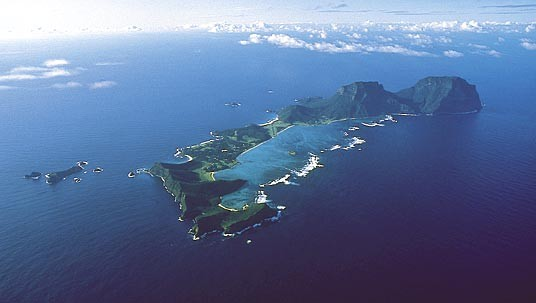
\includegraphics[scale=0.5]{img/LordHoweIsland2.jpg}\\[4mm]}
%%    \par
%%    
\includegraphics[scale=0.1]{img/vk9l-w7brs.png}}
\label{theislandtitle}
\end{minipage}
\\[1cm]
Scoping Document for Expedition\\[1mm]
{\small{Rev 1.25}}\\[2mm]
July {20{\textsuperscript{th}}} - August {1\textsuperscript{st}}, 2024\\[1cm]
}

\begin{document}

\maketitle

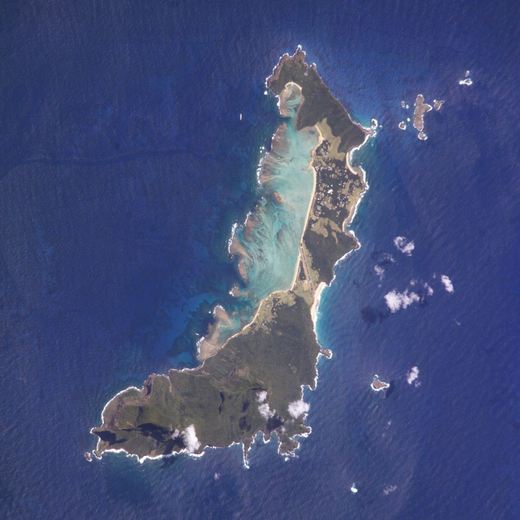
\includegraphics[scale=1.0]{img/520px-Lord_Howe_ISS006-E-5731.png}
\par

\begin{abstract}
The goal is to reach Lord Howe Island and operate for
a couple of weeks on as many {\gls{hf}} bands to give the amateur radio
community an ``activation'' of a semi-rare entity.  This Plan is
the outline and details which cover the objectives,
methods and tasks to perform.  This document is the governing document
for how and what this DX'pedition is for Lord Howe Island.
\end{abstract}
\clearpage

\begin{acknowledgements}
Special acknowledgement to the following:
\begin{itemize}
\item Tom Berson, {\qrz{ND2T}} for the outline of a DX'p plan.
Much of the content is based on his talk about DX-peditions at Visalia
2023.
\item Charles ``Rusty'' Epps, {\qrz{W6OAT}} for his friendship and 
mentoring me in all areas of DX, contesting and reminding me to keep having fun.
\item Mark Aaker {\qrz{K6UFO}} for his support and advice and good talks
over a glass of wine.
\item Al Rovner, {\qrz{K7AR}} and Bob Norin, {\qrz{W7YAQ}} for their advice and information about Lord Howe Island.
\item Bob Schmieder, {\qrz{KK7EK}} for his inspiration to follow my {\textit{DX-Aku}}.
\item To the rest of the clubs, foundations and organizations that
inspire us to chase DX and be the DX, thank you.
\end{itemize}

\end{acknowledgements}
\vskip2cm
\section*{Contact}
The author can be reached via email at {\texttt{jdw@w7brs.com}}.\\[1cm]
Telephone at: {\texttt{+1 425 394 9990}} (Pacific time please).\\[5mm]
Posted materials sent to:\\[4mm]
ARS VK2/W7BRS\\
c/o Jeff Wandling\\
27801 SE 43rd PLACE\\
FALL CITY, WA 98024\\
U.S.A.\\
\par
\noindent
Web address for DX'pedition will be posted soon.
\par
\noindent
In mean time, this document will be regularly and frequently updated.
Please find this document at the following address:\\[3mm]
\noindent
\href{http://w7brs.com/vk9l/scope.pdf}{Lord Howe Scope Document}\\[3mm]
\noindent
A summary web page template is under development and can be found at:\\[3mm]
\noindent
\href{http://w7brs.com/vk9l}{VK2/W7BRS Expedition Page}\\[3mm]
\par
\newpage

\tableofcontents
\listoffigures
\listoftables

\newpage
\section{How to Read this Document}

This document is a draft plan for an DX'pedition happening in July
of this year.   There are many instances in this document of the term
{\texttt{TBD}} and {\texttt{TBR}}. 
\begin{itemize}
\item {\texttt{TBD}} is To be Determined.  It may not apply or it may apply.
\item {\texttt{TBR}} is To be Reviewed. It will apply, but the details
are uncertain.
\end{itemize}

{\texttt{TBD}} could be removed. {\texttt{TBR}} will remain until the
uncertainity is resolved.

Hypotheticals:
\par
\begin{enumerate}
\item {\textit{``The operation will use FT-4, TBD.''}}   Meaning: we may or we may not use FT-4.  If we decide not to, then that hypothetical statement will be removed.
\item {\textit{``The operation will use FT-8, FT-4, TBR.''}}   Meaning: we may or we may not use FT-4 or FT-8, but the list of what digital modes we do use
will be reviewed until that uncertainity is removed.
\item {\textit{``The operation will work on 80-10 meters, TBR.''}}  Meaning: we may not use all of those bands, but we are using bands and the list will be reviewed until that uncertanity is removed.
\end{enumerate}
\par
Thanks for your understanding.

\newpage
\section{Preliminaries}

The geological setting for Lord Howe Island is 580 km off the coast
of Australia upon the western edge of the Lord Howe Rise.

\par
The Rise is a continental ribbon, rifted from eastern 
Australia during the Crataceous to Paleogene and
forms a submerged portion of the microcontinent
Zealandia.\cite{lhi}
\par
According to geological studies what remains today is a 
a remnant of an eroded shield volcano that 
erupted between 7 and 4 million years ago. 
\par
The age of of the island and the seamounts in the region are less in the
south which suggests that the a northward trajectory of the Australian plate
over a stationary mantle plume.
\par

A set of reference maps that detail the interesting geology are included
in the appendix.


\section{Scope}

\vskip2mm
\noindent%
\begin{minipage}{\linewidth}%
\makebox[\linewidth]{%
    
\includegraphics[scale=0.5]{img/300px-Flag_of_Lord_Howe_Island.svg.png}}
\captionsetup{width=0.8\linewidth}
\captionof{figure}[Flag of Lord Howe Island]{Flag of Lord Howe Island}
\label{flag}
\end{minipage}
\vskip5mm

The DX'pedition to Lord Howe Island is a solo trip by the author, Jeff
Wandling, W7BRS.  The basic information about the trip is summarized
in the list below.

\begin{itemize}
\item {\textbf{Call: VK2/W7BRS}}
\item {\textbf{What: A {\gls{flyin}} DX'pedition to Lord Howe Island}}
\item {\textbf{When: {\gls{qrv}} July 20th through August 1st, 2024}}
\item {\textbf{Where: QTH Beachcomber Lodge, Lord Howe Island, Australia}}
\item {\textbf{{\gls{iota}}: OC-004}}
\item {\textbf{Continent designation: Oceania}}
\item {\textbf{ITU: 60, CQ: 30, DXCC: \#147}}
\item {\textbf{Bands: 40m through 10m, CW, FT8 and SSB}}
\item {\textbf{QSL: ClubLog OQRS and LotW (pending)  \ldots}}
\item {\textbf{Operators: Jeff Wandling, W7BRS /  \ldots}}
\begin{itemize}
    \item ClubLog Most-Wanted\footnote{As of April 2024}: \#63
    \item Will be QRV during {\gls{rsgb}} IOTA CW contest.
\end{itemize}
\end{itemize}
\par

\vskip2mm
\noindent%
\begin{minipage}{\linewidth}%
\makebox[\linewidth]{%
\includegraphics[scale=0.3]{img/beach-comber-lodge-qth.png}}
\captionsetup{width=0.8\linewidth}
\captionof{figure}[Site Terrain]{The site terrain of the QTH is located
on a farm on the northern leg of the island.
The Plan is to go to {\gls{lhi}} and operate HF for approximately
two weeks from the site Beachcomber Lodge located on the northern
tip of the island.}
\label{farm}
\end{minipage}
\newpage
\vskip4mm

\noindent%
\begin{minipage}{\linewidth}%
\makebox[\linewidth]{%
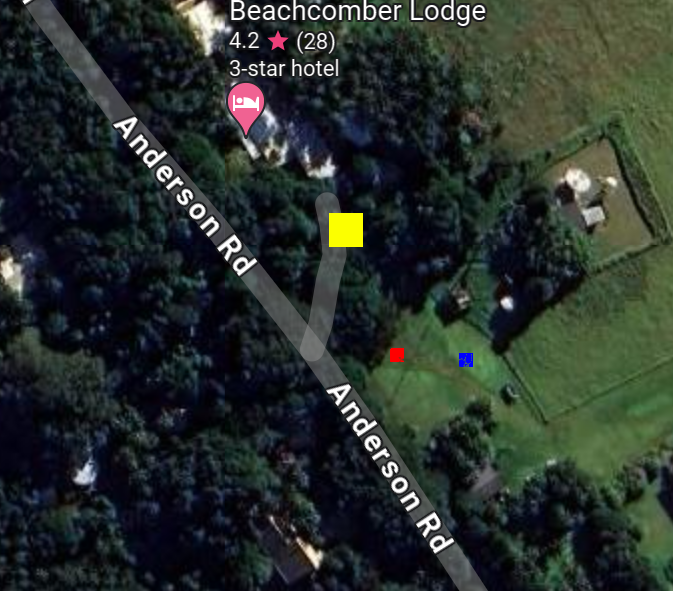
\includegraphics[scale=0.5]{img/beach-comber-lodge-qth-ant-loc.png}}
\captionsetup{width=0.8\linewidth}
\captionof{figure}[Shack and Antenna Location]{
The yellow box represents the location planned for the shack.  The
red and blue boxes represent the approximate location of the vertical
antennas deployed -- DX Commander and SteppIR {\gls{crankir}} vertical}
\label{ant-farm}
\end{minipage}
\newpage
\vskip4mm

\subsection{Important Checklist}

\vskip2mm
\noindent%
\begin{minipage}{\linewidth}%
\makebox[\linewidth]{%
\begin{tabular}{|l|l|} \hline
\checkmark & Secured Immigration Visa for Australia \\ \hline
\checkmark & Airline tickets purchased \\ \hline
\checkmark & Reservations made for site lodging \\ \hline
\xmark     & Final antenna inventory \\ \hline
\xmark     & Public Announcement \\ \hline
\end{tabular}}
\captionsetup{width=0.8\linewidth}
\captionof{figure}[Main Issues]{Most pressing tasks to resolve soon.}
\label{pressing}
\end{minipage}
\newpage

\subsection{Where Is Lord Howe?}

\vskip2mm
\noindent%
\begin{minipage}{\linewidth}%
\makebox[\linewidth]{%
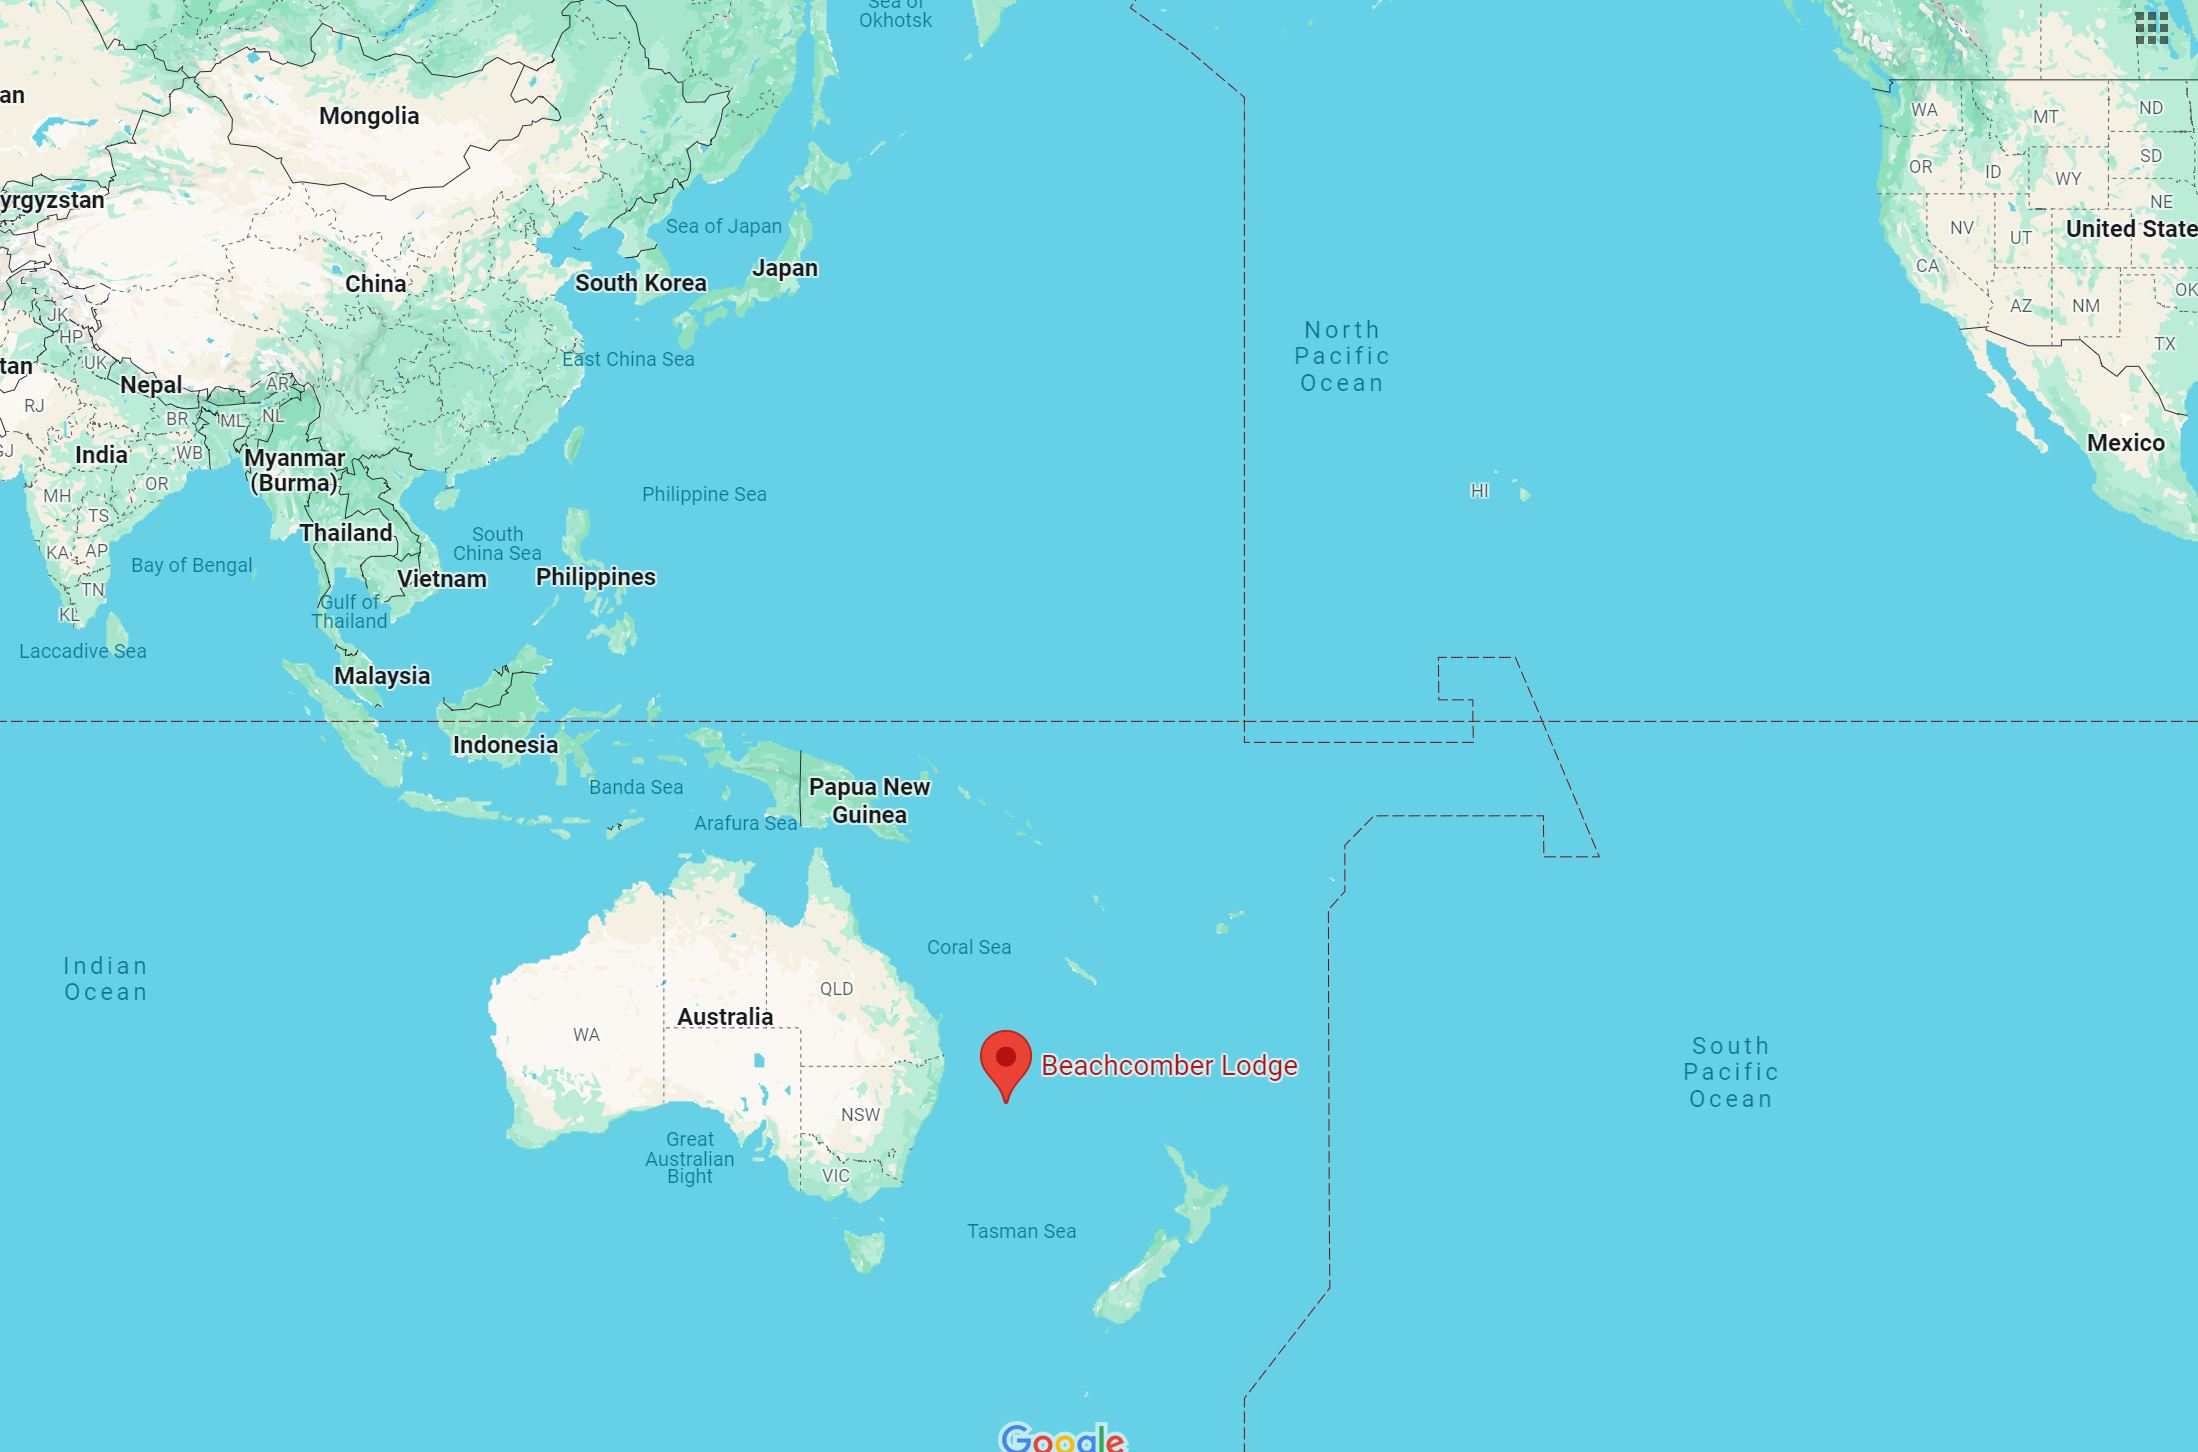
\includegraphics[scale=0.5]{img/Oceania+LordHowe+Island.JPG}}
\captionsetup{width=0.8\linewidth}
\captionof{figure}[Location]{Proximity of LHI with Australia and the North American, South American and Asian continents.}
\label{prox}
\end{minipage}
\vskip3mm

\par
LHI compares with these other sought after entities, for example:
\vskip2mm

\noindent%
\begin{minipage}{\linewidth}%
\makebox[\linewidth]{%
\begin{tabular}{|l|l|l|} \hline
Rank & Prefix & Entity \\ \hline
{\textbf{63}} & {\textbf{VK9L}} & {\textbf{Lord Howe Island}} \\ \hline
66 & CY0 & Sable Island \\ \hline
70 & 7O & Yemen \\ \hline
93 & HV & Vatican City \\ \hline
139 & YA & Afghanistan \\ \hline
174 & S7 & Seychelles Islands \\ \hline
198 & CE9 & Antarctica \\ \hline
\end{tabular}}
\captionsetup{width=0.8\linewidth}
\captionof{table}[Rank of VK9L]{Comparison of VK9L with other sampled DX entities for
comparison.}
\label{compare}
\end{minipage}

\section{Geography}

\vskip2mm
\noindent%
\begin{minipage}{\linewidth}%
\makebox[\linewidth]{%
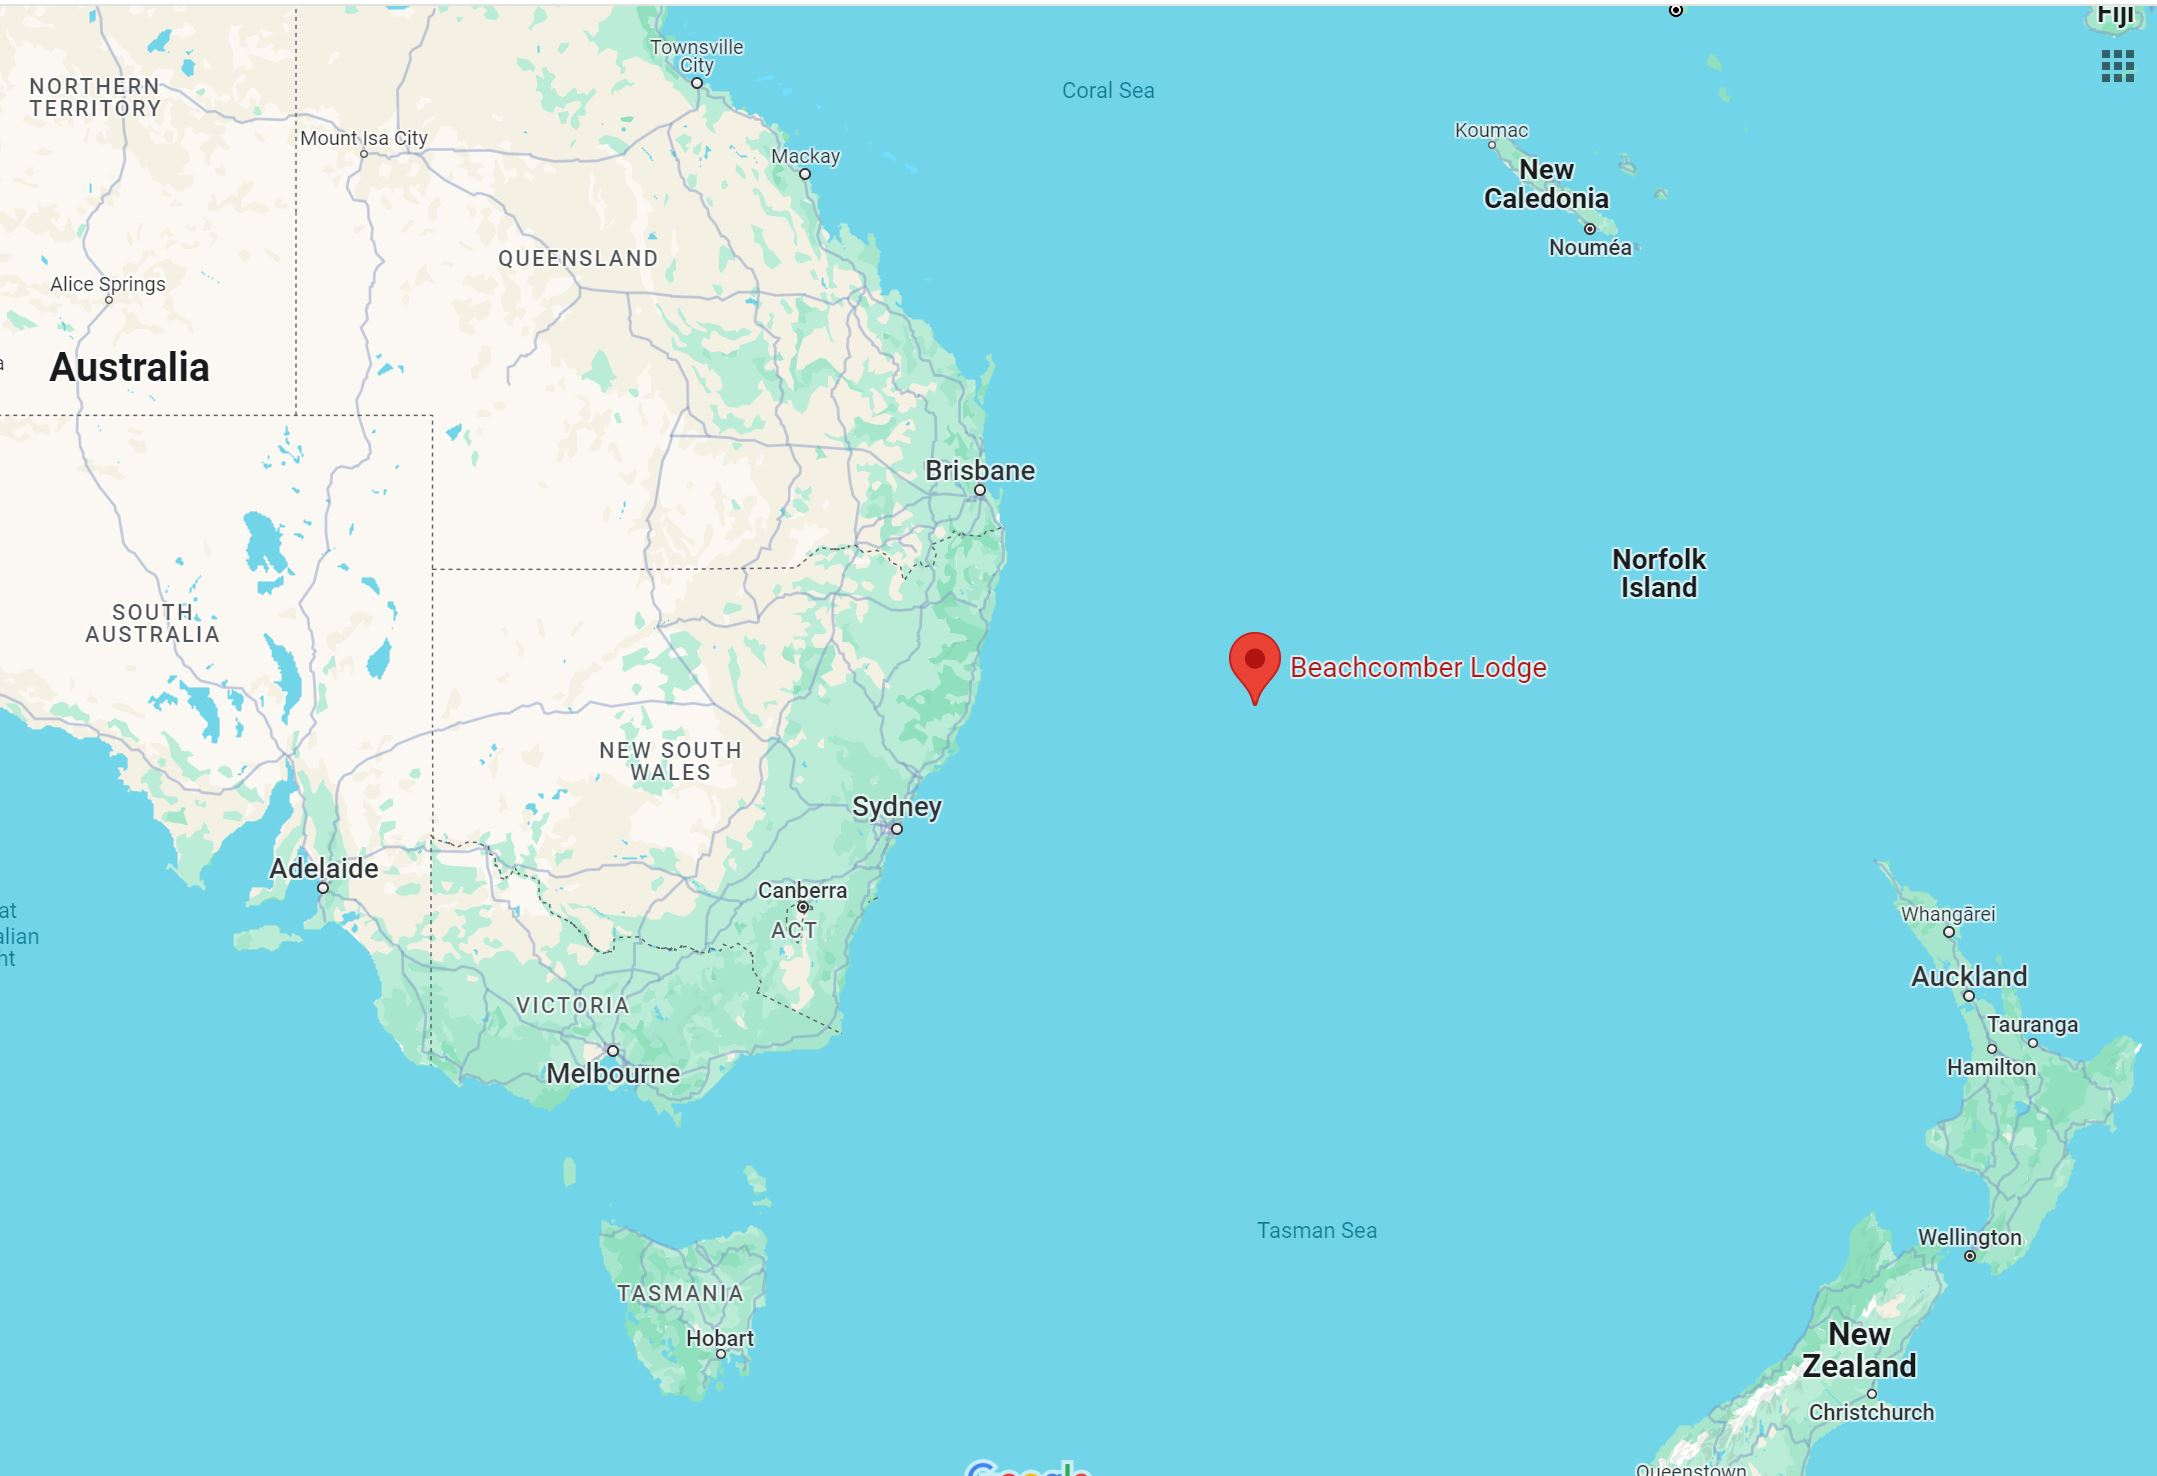
\includegraphics[scale=0.5]{img/Australia+LordHowe+Island+Proximity.JPG}}
\captionsetup{width=0.8\linewidth}
\captionof{figure}[Nearby Countries]{Location of Lord Howe relative to Australia and surrounding
islands in Oceania.}
\label{location-relative}
\end{minipage}
\vskip3mm

\noindent%
\begin{minipage}{\linewidth}%
\makebox[\linewidth]{%
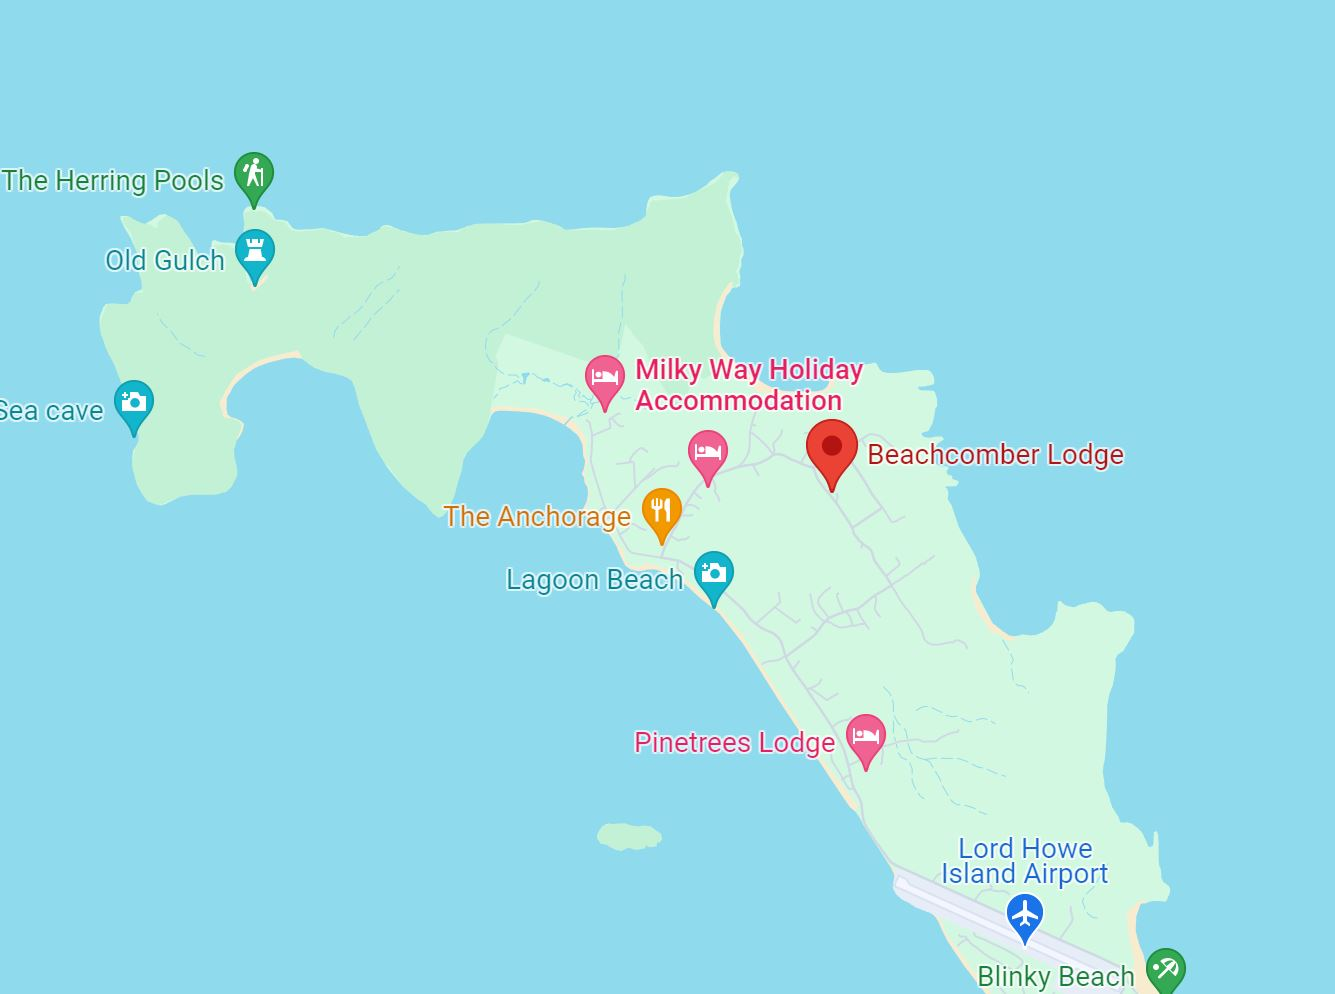
\includegraphics[scale=0.8]{img/BeachcomberLodge.JPG}}
\captionsetup{width=0.8\linewidth}
\captionof{figure}[QTH]{Location proposed on LHI -- The Beachcomber Lodge.}
\label{location-relative-qth}
\end{minipage}
\vskip3mm


The Azimuthal map (attached) will show that amateurs located in North America,
East Asia, and Europe will be reachable with an array of antenna that are pointed almost due North from the island.  Contacts to South America and Africa will
be reachable with a different orientation of the antennas.

\vskip2mm
\noindent%
\begin{minipage}{\linewidth}%
\makebox[\linewidth]{%
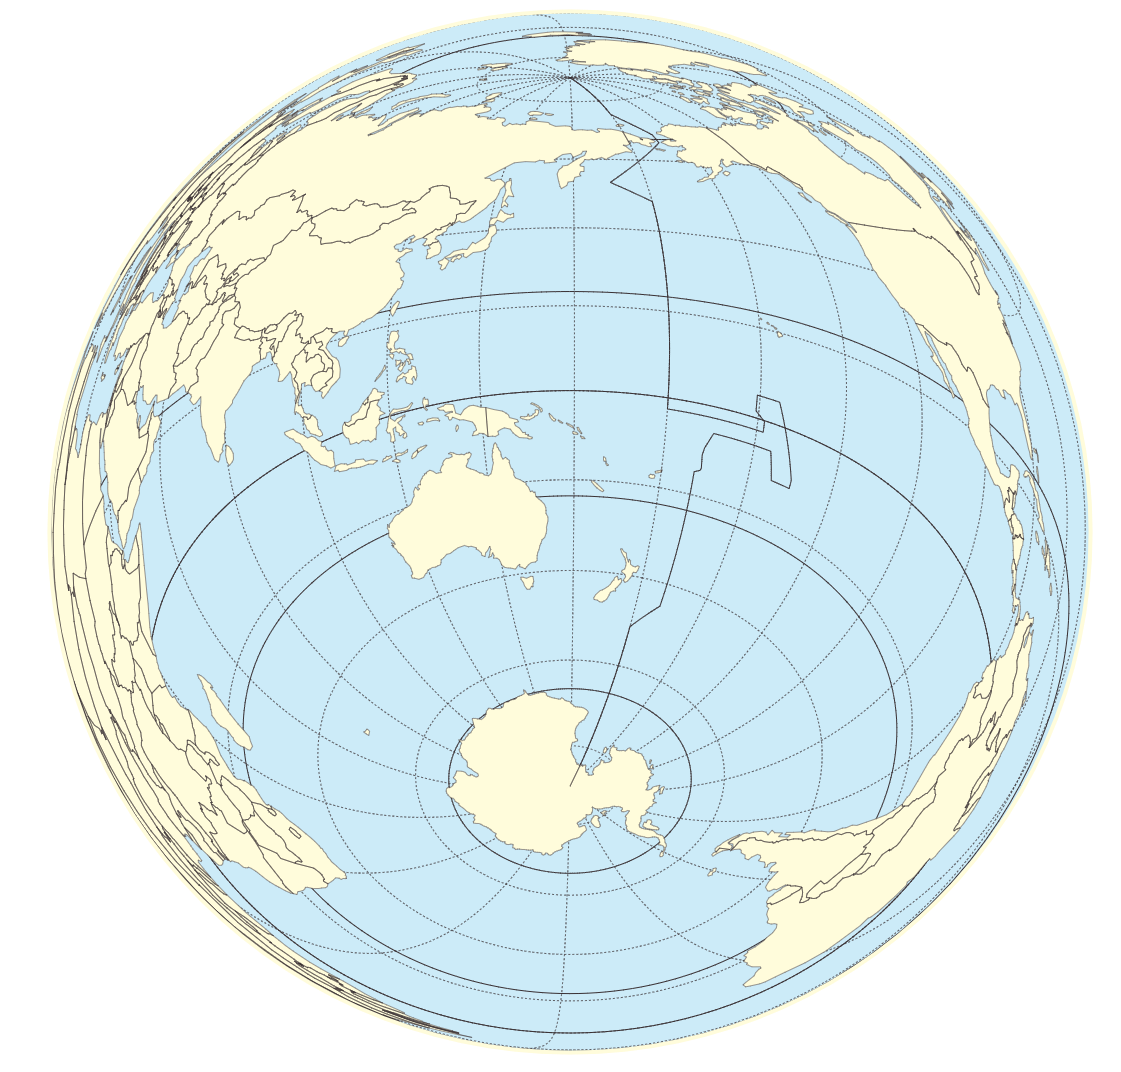
\includegraphics[scale=0.5]{img/azimuth.png}}
\captionsetup{width=0.8\linewidth}
\captionof{figure}[Azmuthal Map]{Approximate Azmuthal headings for LHI
for the main target operations of NA, JA (Asia) and EU}
\label{azim}
\end{minipage}
\vskip3mm

\section{Weather}

It is going to be cold on LHI.  For the standard weather
the author is used to in the Seattle area, the weather is actually
on par with a typical early spring or early fall day.  Mid 60's (F)
and frequent rain.  Not a bad weather event for the Seattle area,
but it will be chilled weather nonetheless. 
\par
Aside from the dynamic effect on the antenna tuning, the weather
will require a set of warm clothing and rain-gear.  Winds are 
expected, so rigging to keep the antennas up are required.

\vskip2mm
\noindent%
\begin{minipage}{\linewidth}%
\makebox[\linewidth]{%
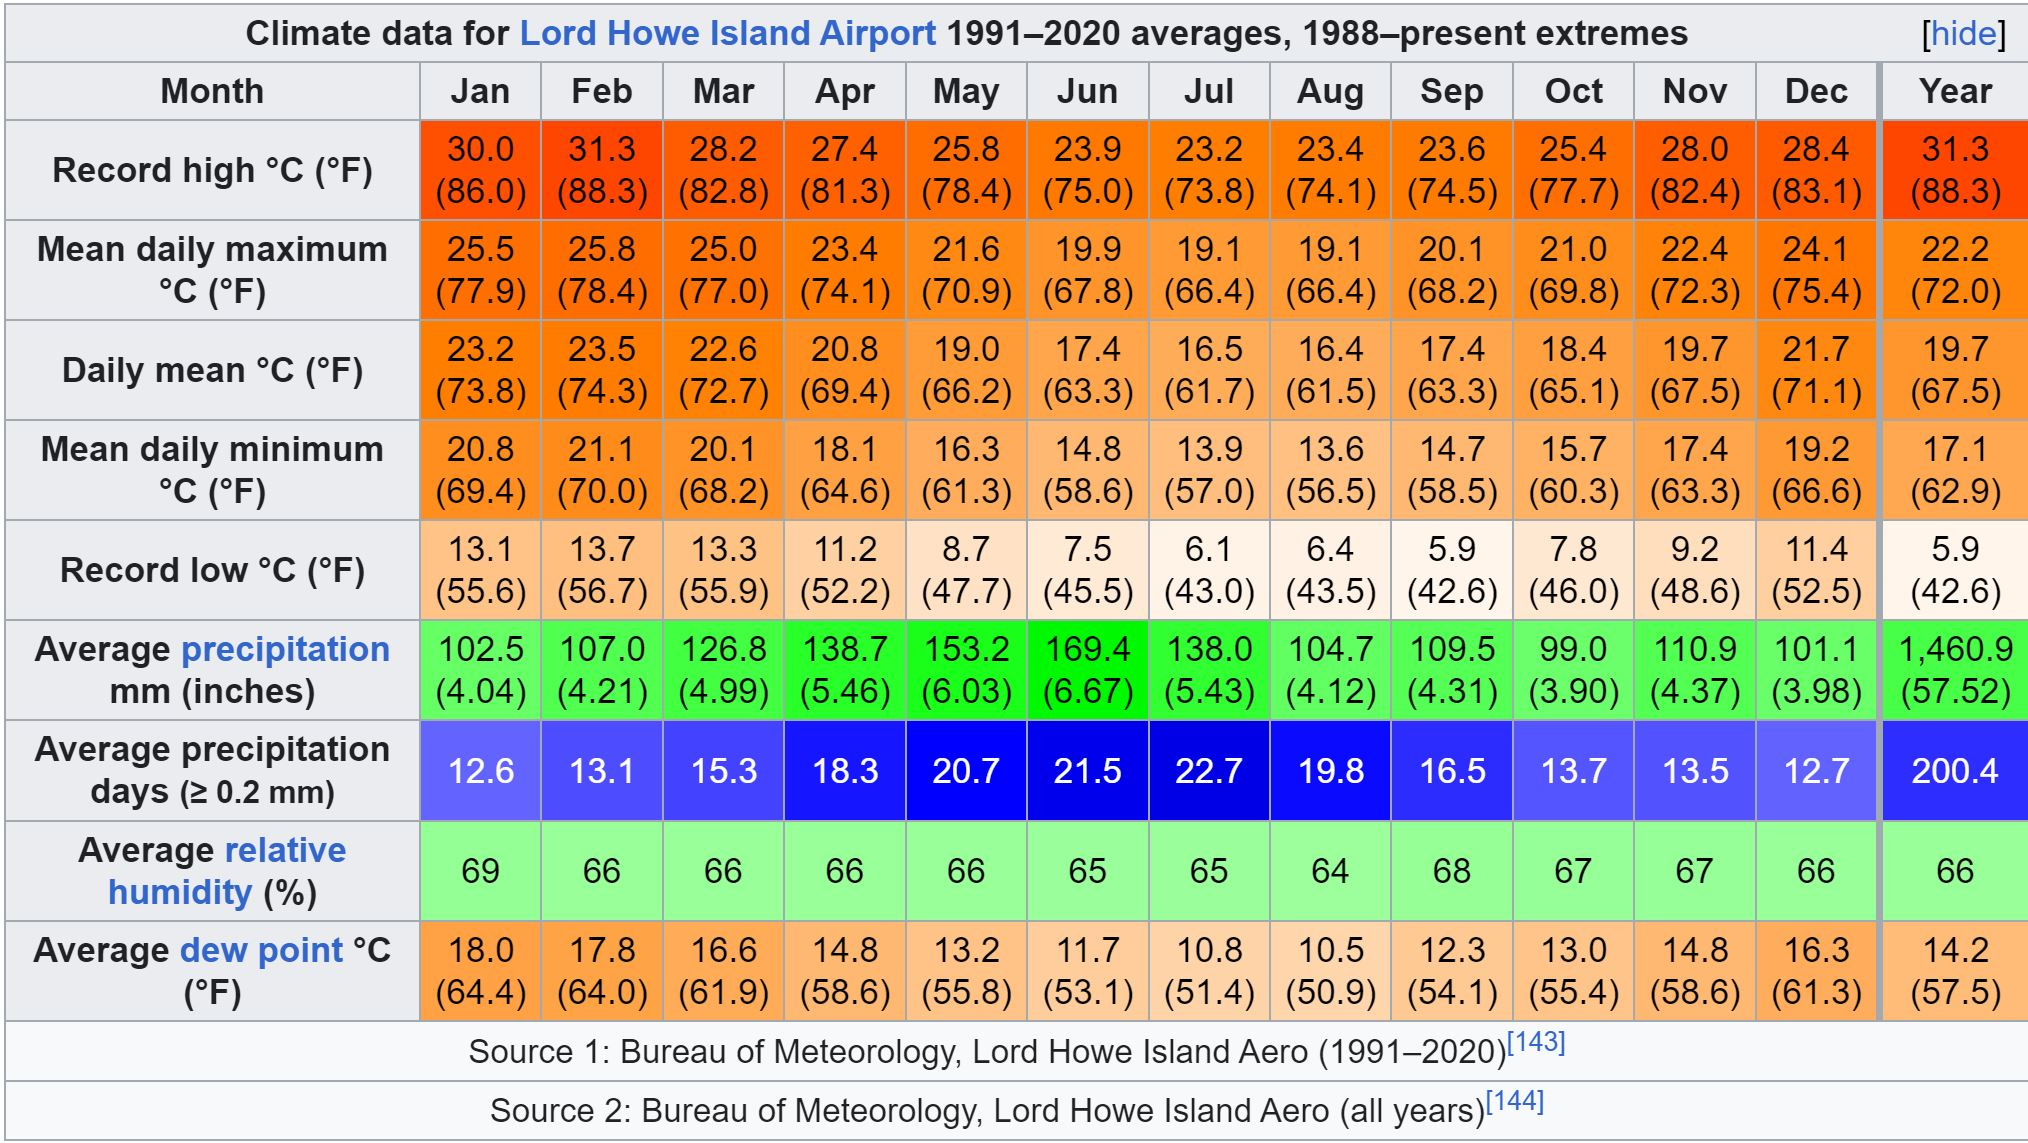
\includegraphics[scale=0.6]{img/weather-chart-vk9l.JPG}}
\captionsetup{width=0.8\linewidth}
\captionof{figure}[Weather Pattern]{A weather chart showing trends of temperature,
rainfall on Lord Howe Island.}
\label{rain}
\end{minipage}
\vskip3mm

The expectation is a colder-than-normal Seattle type weather situation.
\par
Warm clothes, and layers is the recipe to deal with that.  It will not
be a huge difficulty to overcome.

\section{Goals}

The goal of the expedition is to activate a semi-rare island
during a upward trend in solar cycle 25 when propagation should be
at a good level for reaching most amateurs who need LHI.
\par
The lesser goals are
\begin{enumerate}
\item Make this an adventure for the DX-pedition.  The island is
nearly on the far side of the globe from where the organizers reside.
It's below the equator from the most populated areas with amateur
radio operators (North America, East Asia and Europe).
\item To make as many QSO as time permits.  The
goal to make good rate for QSO is underlying all of the
other goals, but there will be challenges to reach
modest numbers given the level of experience with 
pile-ups and DX'peditions.
\item The rare qualities of the island make it suitable
for a DX'pedition.  It's semi-rare, but difficult to
reach despite the proximity to the mainland of
Australia.  It's mostly known as a tourist destination
however there is unique history to the island.  There
have not been frequent trips to LHI.
\item Follow the rules of the ARRL DXCC whereby
the entity will count for LHI on
the bands that are worked.
\end{enumerate}

\section{Type of Expedition}

These are the qualities of the VK9L expedition:
\vskip2mm
\noindent%
\begin{minipage}{\linewidth}%
\makebox[\linewidth]{%
\begin{tabular}{|l|l|} \hline
{\textbf{Status}} & {\textbf{Attribute}} \\ \hline
\checkmark & {\gls{singletwo}} \\ \hline
\xmark & {\gls{multisingle}} \\ \hline
\xmark     & Vacation \\ \hline
\cmark     & Contest \\ \hline
\checkmark & Activation \\ \hline
\xmark     & Heavyweight \\ \hline
\checkmark & Lightweight \\ \hline
\xmark     & 5-Star \\ \hline
\checkmark & 3-Star \\ \hline
\checkmark & {\gls{flyin}} \\ \hline
\xmark     & Tent and Generator \\ \hline
\checkmark & Verticals \\ \hline
\xmark     & {\gls{beam}} and Rotators \\ \hline
\end{tabular}}
\captionsetup{width=0.8\linewidth}
\captionof{table}[Type of Expedition]{Metrics about this DX'pedition.  The bias
is on a simple compact DX'pedition.  No reliance on pre-shipping
or advanced antenna systems.  No reliance on generators, tents
or other means to survive in harsh climates and conditions.}
\label{typeof}
\end{minipage}
\vskip3mm

\section{VK9L Leader Roles}

This expedition is not initially planned as a multi-op Team, however 
to lay the ground work for future expeditions, the template for
Leader and Planner roles are defined as follows.  
\par

The roles contemplated at this stage of planning are as follows:

\begin{itemize}
\item Leader and Organizer
   \begin{itemize}
      \item Jeff Wandling, W7BRS
      \item TBR\ldots
   \end{itemize}
\item Operator(s)
    \begin{itemize}
      \item Leader
      \item TBD\ldots
    \end{itemize}
\item Implementation -- Each of these categories themselves is a sub-team (1 to $n$ people).
     \begin{itemize}
         \item Fund-raising --  \ldots
         \item PR and Marketing --  \ldots
         \item Food and Lodging --  \ldots
         \item Property Master (equipment, location, facilities) --  \ldots
         \item Power Systems --  \ldots
         \item Antenna design and deployment --  \ldots
         \item Station Setup (Transceiver, PA, Peripherals) --  \ldots
         \item Software and Networking --  \ldots
         \item Media and QSL Content (ClubLog, LiveStream, {\gls{lotw}},
 {\gls{qsl}}) --  \ldots
         \item Tear-down and Removal --  \ldots
     \end{itemize}
 \end{itemize}

As shown the list of things to span across the range
from organizing to implementation.  On a team-effort expedition,
those roles would be assigned to specific sub-unit leads.
\section{Tasks}

The following outline the tasks that must be performed.

\subsection{Vision}
   The Vision ties into the overall goals of the expedition and serves
the purpose to develop PR and Marketing materials for the presentation
and solicitation of support from the amateur radio community and 
commercial entities for equipment and monetary support.
\par
In addition, several DX Clubs and Foundations are involved in 
shaping the vision to some extent by consultation with experts
for generating the most compelling and exciting expedition Plan.
\par
The vision of this expedition is to lay the ground work for future
expeditions by making an exercise onto a relatively uncommon location
for DX.   A lot of the issues are present that would be on any other
expedition -- even those of more severe risk and cost.  It is fully
understood though that {\textit{this}} expedition does not share
the same amount of danger, cost or consequence as many very
complicated expeditions.  To name a few -- {\texttt{H44WA}}, {\texttt{TX5S}},
etc\ldots.  Those expeditions had challenges that do not occur on
Lord Howe Island (heat is not a factor, abundant animal wildlife
intruding on the operating site is also not expected).
\par
Aside from the objective vision of setting out for an adventure
to experience the DX'pedition first hand, the author has developed
the vision to embrace a few things that have been collected by readings
and interviews with other DX'pedition experts.
\par
Here is a quick list of those elements of the vision.
\begin{itemize}
\item Nothing is what it seems.  Trying to understand the issues
that occur on a DX'pedition can not only be learned by reading and talking
to those who have done these trips.  It's apparent that simply 
reading and talking about DX'peditions is not enough.  The vision therefore
is to immerse into the role and activities that are likely to be common
for any DX'pedition.  {\textbf{The vision charts a course towards
better understanding of real-world situations that could occur on
any typical DX'pedition.}}  Perhaps even the phrase
{\textit{any typical}} is misplaced.  Perhaps there is no such thing
as a {\textit{typical}} expedition.  Part of the vision then is to
gain a better perspective if that is indeed the case.
\item ``Do what you know how to do.'' Those were the words
from the fictional muse in Schmieder's book.  Through a concentrated
filter, the book introduces a basis for DX'peditions that is centered
around a couple of points that overlap with this author's own perceptions.
   \begin{enumerate}
     \item {\textit{Do what you know how to do.}}  Keeping the operation
simple, keeping the goals simple and staying within the domain of 
experience and knowledge that contributes to success.  For example, the
author has no experience with {\gls{eme}}  operations.  So
this expedition will not do EME.   We will not work satellites either,
even though the author has experimented with it.  Experimentation versus
dedicated experience is the factor to determine what we do.
    \item Demonstrate that even the new DX'peditioner can be successful.
One of the comments I heard when discussing this plan was ``No one knows
who you are.''   The author does not necessarily want to negate that
perception.  The author is fine not being known, but the impact of not
being known means that for the most part -- any requests for support,
advice or -- really anything -- are virtually ignored.   There is
{\textbf{zero probability}} that this author is going to call up
{\textit{DX Engineering}}, or {\textit{Elecraft}}, or any other
source of most serious DX'pedition gear and {\textit{ask for anything.}}.
\par
It will not happen.
\par
The reason it will not happen is that the author is not known.  The author is
not a DX'peditioner.   So the vision of {\textit{this adventure}} to LHI
is to resolve that question -- can a new DX'peditioner become known?  Should
they?   Does it help to do DX'peditions on your own (solo) in order to
become proficient enough to work with other teams when those other teams
do DX'peditions?
\par
Part of the vision of this trip is to find out.
\end{enumerate}
\item  For the purpose of bringing the world a little closer, make an effort
on the island to document very special things about Lord Howe Island.  For
example the Leader plans to have casual interviews with as many people
who reside there -- to get a sense of what they like about LHI, how
they feel about the special nature of the island, and to gather 
interesting stories of the remote past.   Combined with those interviews
also visually document the affair and collect photographs of places,
events and people that are seldom seen from the outside world.  It is not 
a vision to attract {\textit{more visitors}}.  The population dynamics
of the island are already very delicate and precise with respect to
how many people can be supported on the island (resident and tourist).
\par
The best analogy here is the {\textit{National Geographic}} approach
to find something novel and interesting as much as possible -- document it,
photograph it, record the audio, and bring it back to the public in 
a compelling way to express the beauty of the natural world and the humanity
is on Lord Howe Island.
\end{itemize}

There is not going to be an effort to push the envelope with respect
to technology and develop new mechanisms for handling a DX'pedition.
The last several years has seen an explosion of technology rush
through the ham shacks across the world.   First and foremost -- the 
revolution of digital modes via FT-8 and the hybrids.   It is not that
digital modes are new.  They are not.  In fact they are quite old
in terms of the history of amateur radio.  Phased Shift Keying has
been around since the late 30's - 40's.  

\par
But, the software
(another aspect of amateur radio to address) has made it virtually
``point and QSO''.  The author is a software engineer by training.
From that perspective, using software is a classic case of developing
a tool-set to make tasks that used to be complicated much easier and
routine.   We've seen that be the case for quite some time.  A few
examples -- Log Book of the World.   It used to be difficult to 
maintain a database of QSL for important QSO. Now it's literally
embedded into logging software (another benefit) to adjust
counts of {\gls{atno}}.
\par
Digital modes likewise, with the wonderful features of {\gls{wsjtx}}
have made it incredibly easier to work a good DX station.   Digital
modes like FT-8 do not completely level the playing field, but they
make the playing field a lot less bumpy and uneven.
\par
So to that extent, the expedition Vision for this LHI activation
is not necessarily bound to a set of rules to push the envelope of
technology further out.  That level of frontier crashing development
takes years of planning and truly inspirational thinking by those
(and a team) to develop those initiatives.   Still, incremental
improvements are a hallmark of any good study of Amateur radio and
(perhaps with a wink), the author may put something into this
trip that exercises some novel approach to DX'peditions.
\par
Some ideas along the lines of
\begin{itemize}
\item Reproduce the simplicity of Anti-{\gls{dqrm}} techniques in digital modes.
A new baseline of WSJT-X has been released that offers some features
to establish authenticity to the QSO from a prospective DX station.
\item Further lift the curtain to show just how much work needs to
go into a DX'pedition -- not to discourage, but provide inspiration.
To that end, perhaps (since the author likes to write), a series of 
semi-non-fiction stories will be generated.   The amateur radio
DX library may be getting a tad dusty in the last 10-15 years.
\end{itemize}

\subsection{Landing Permission}

Due to the geopolitical nature of the island, landing on the island is
purely a commercial enterprise -- just flying to LHI
is easy as booking a flight.  However, since the island is dominated
by tourism in a way, ``landing'' permission entails finding a location
on the island that would permit radio operations.   The impact
of the expedition on other guests of the island is probably the most impact
and requires the most sensitivity when addressing the goal of finding
the ideal location.

\par
The equation with factors that decide optimal location, and thus
drive the need for specific ``landing'' permission are to be covered
throughout this Plan.  But, at the basic level there appears to be
a bias forced by the Island that the location is NOT going to be near
salt-water but rather on elevated terrain within a mile of salt-water.
\par
We will cover the impact and benefits of this bias throughout the
Plan.

\subsection{Licensing}

Licensing is through the Australian government.

\par
The reciprical agreement permits the use of {\texttt{VK2/W7BRS}}
without a separate license.
\par
As long as the requirements are met for the US license holder
to operate in Australia on the bands and modes limited to
Australian {\textit{Advanced}} class license (which is effectively
equivalent to the {\textit{Extra}} class) notwithstanding the 
band restrictions (such as 60m), the prosign call is allowed.

\subsection{Team Building}
The Team is built by recruiting knowledgeable operators who have
distinct skills that overlap.   Every operator should have
at least operational skill in handling the basic features of
the radio equipment (split, filtering) phonetics, timing,
economy with QSO patterns, logging software, and patience.
\par
Most of all Team members need to have innate awareness of
working pile-ups, and patience to stick to the operational
goal for the session (i.e., work NA or work JA's or work EU
as the band and openings dictate).
\par
In addition to building a Team based on skills and performance,
another set of factors include
\begin{itemize}
\item General Health
\item Ability to deal with adversity
\item Stamina to work and sleep at odd-hours for days
\item Able to cope with a bland diet
\item Cheerful under the pressure of typical stress encountered
in a unfamiliar place -- society, terrain, weather, odd working
conditions -- time of day, sleep deprivation, adapting to 
{\textit{followership}} -- sticking to a plan, constructively 
discussing changes, and when necessary disagree but commit to what
the Leader ultimately suggests.
\end{itemize}

The Team is going to need to focus on key areas

\begin{itemize}
\item Basic first-aid
\item Fund-raising
\item PR and Marketing
\item Plan checking and brainstorming
\item Communications on site (HT, Repeater on-site)
\item Knowledge of and skill at CW
\item Knowledge of and skill at SSB
\item Knowledge of and skill with FT-8 (hybrids too)
\item Antenna deployment, tuning and adjustment
\item Station layout, connections, features
\item Food and Shelter
\item Logistics, scheduling, team morale
\item Risk mitigation, safety, security
\item Logging, Software, Networking, Integration with Services
\end{itemize}

\par

The solo operator for this LHI operation has a good background
in the following necessities (where checked) on a scale of 1-10:
\vskip2mm

\noindent%
\begin{minipage}{\linewidth}%
\makebox[\linewidth]{%
\begin{tabular}{|l|l|l|} \hline
{\textbf{Satisfied?}} & {\textbf{Level 1-10}} & {\textbf{Attribute}} \\ \hline
\cmark & 10 & First-aid and CPR \\ \hline
\xmark & 1 & Fund-raising  \\ \hline
\xmark & 1 & PR and Marketing \\ \hline
\cmark & 8 & Plan checking and brainstorming \\ \hline
\cmark & 8 & Communications on site (HT, Repeater on-site) \\ \hline
\cmark & 7 & CW (25 w.p.m contesting, 18 w.p.m rag-chew) \\ \hline
\cmark & 9 & SSB \\ \hline
\cmark & 9 & FT-8 (hybrids too) \\ \hline
\cmark & 9 & Antenna deployment, tuning and adjustment.  \\ \hline
\cmark & 8 & Station layout, connections, features \\ \hline
\cmark & 7 & Food and Shelter \\ \hline
\cmark & 7 & Logistics, scheduling, team morale \\ \hline
\cmark & 6 & Risk mitigation, safety, security \\ \hline
\cmark & 9 & Logging, Software, Networking, Integration with Services \\ \hline
\end{tabular}}
\captionsetup{width=0.8\linewidth}
\captionof{table}[Operator Evaluation]{Self evaluation of the author's skills on
various roles and abilities on the expedition.}
\label{eval}
\end{minipage}
\vskip3mm

If this was a Team event, each member should have an overlap of 
two or three (or more) areas
of expertise. \par
For example a team member of value would
have a combination of three or more features like:

\begin{itemize}
\item Plan checking and coordination, Knowledge of SSB, Antenna setup.
\item Another Team member may have more experience that covers a broader
range like:  CW, SSB, Safety and Software, etc \ldots
\end{itemize}

\subsection{Budget}

The two main cost centers for the expedition are

\begin{itemize}
\item Flights - approx. \$3,000 (RT) from SEA.
\item Lodgings - approx. \$3,400 (10-12 nights) on LHI.
\item Capital investment \$3-4,000 (antennas, cables, electronics,
rigging, travel containers
\end{itemize}

The budget therefore per person is roughly \$7-10,000 if all 
of the other incidentals are taken into account.
\par
There are capital costs for setup and equipping the expedition.
There are consumables and non-recoverable costs (food, 
flights, lodgings, etc\ldots)

\par
A complete breakdown is not yet established, but the estimate
(which will likely increase) is around \$10,000 per person, not 
including the capital investments.

\subsection{Fund-raising}

Fund-raising is an action to take at three different phases of the
expedition.

\begin{itemize}
\item Before -- during the stage from Planning until Announcement
funds will be needed from stake-holders who are friendly to the
Plan.   DX Foundations, Clubs, Vendors, Commercial entities,
and private donations.
\item After announcement until departure will seek small
numerous donations from the general amateur radio public.  This
seems to be the make-or-break inflection of the whole operation.
Unless {\textbf{during}} the middle phase enough funds are secured,
then the expedition will not be able to proceed according to this Plan.
A clear cut-off has to be made prior to expenses paid that are 
non-recoverable.   Yet, there may be some expenses that are paid
out that are non-recoverable even in the event of the cancelation
of the expedition.
\item During on-island and post expedition phase -- where 
appreciated support during the well run expedition is expected.  In
addition, {\gls{oqrs}} may contribute a small portion to the
income to cover costs already paid and fund the distribution of
QSL.   ``Swag'' is also something that will be offered -- both
in the spirit of celebrating the expedition, but also (with the
Vision and PR/Marketing ideas) emphasize the island itself.
In a time and age of increased awareness of environmental
impact and climate change, anything (everything) that can be
done to highlight the beauty and magnificence of the Island
may draw in more appeal than simply trying to re-pay
a Expedition Team for their hobby.
\end{itemize}

More, TBR\ldots

\subsection{Transportation}

The route to the LHI site is by air.  Flights route through
Australia.
\par
The flight for the trip originates in Seattle, Washington.
\par
The flight will take two stops (Los Angeles and then Sydney)
before the last hop on DASH-8 aircraft to LHI.

\par
The airlines used are {\textit{Alaska Airlines}}\footnote{
Just for the frequent-flier points.  It does not really
matter which airline is used.  Except -- there are
some anecdotes floating around of certain airlines
in the Pacific presenting problems for DX'peditions.} 
 and {\textit{Qantas}} appears to be the ideal choice.  

\subsubsection{Freight}

There is a need to transport a significant amount of heavy
equipment.  By ``freight'' simply that this equipment is 
a Checked-Bag item:

\begin{itemize}
\item First-aid equipment.  What can make simple problems less difficult?
Pain medication, anti-histamines, digestive aids,  anti-acid,
sleep aids, ace-bandage, sling,
anti-bacterial, cuts and abrasions.  Beyond mild lacerations, advanced
medical {\textit{treatment}} would be necessary.
\item FM/Communications equipment.  Simple HT for the {\textit{host}}
of the site {\textit{and}} the operators of the expedition.  Especially
when first aid is needed and no cell phones are working.  Reaching
the people who are {\textit{not}} part of the expedition who can help
render aid is critical.
\item Backup clothing, backup shelter.  Balance weight and size against
how often it may be possible to re-clean clothes.  Assume the worst --
laundry may not be something easily found.  It may be required to 
find a way to rinse and dry clothes without any services whatsoever.  Expect
``Commando Mode''.
\item Antennas. Compact and extended.  One, maybe two pre-fitted for 40-10m
\item Feed-lines. LMR-240 or RG-8X at correct multiples NOT resonant on
the bands.
\item DC Power supply. Switching, not linear.
\item Tuner. Automatic, plus spare wire for loading coils -- the climate
may present environmental conditions that require the ``pre-fixed'' antenna
to need adjustments.  Radial wire too.
\item Rigging parts. Cinches, guy lines, markers, stakes, flags.
\item Extra food. Just-Add-Hot-Water. \footnote{A personal lesson learned -- always travel with
at least a week worth of freeze dried food ``just add water'' type.
You never know what kind of dietary issues may come up or what
the local cuisine may offer.  A healthy digestive tract is very important,
right?}
\item TBR\ldots
\end{itemize}

What is NOT shipped as freight but carry-on must include

\begin{itemize}
\item Transceivers -- Despite any weight restrictions, these need to
be carried on -- padded, and in 'day packs' so they easily slide under
seats.
\item Amplifiers -- Same story.  Somewhat more rigid, but their sensitivity
is mechanical mostly.  Power supply transformers increase the inertia of the
amplifier and unless the unit is {\textit{designed}} for air-travel
it must not be checked in. $\rho = mv$  Momentum is mass times
velocity. A linear solid state amplifier is 25 lbs.  If the case is ``thrown''
the change in momentum would be destructive for the internal unit.  They are
not made to be thrown.  Carry these on.
\item Hand-Held Transceivers (HT) and related.  These can probably be put into Checked
Luggage actually.
\item The most basic ``Field-Day'' wire antenna solution (in case of the
worst outcome -- that the equipment that was supposed to arrive does not.)
The worst that can happen just might happen. Having a spool of fine wire
in the radio bag can probably turn a trip with zero QSO into one with a fair
showing!
\item A partial-set of the {\gls{tene}} -- extra food, clothing,
and so on within reason.  The site {\textit{is}} a resort after all.
\end{itemize}

It is to be evaluated yet if it makes sense to pre-ship all of the
heavy equipment through a hired customs agent and process so that
before we step onto the plane to LHI, the equipment is already
on site at the operating location waiting for use.

\subsection{Equipment}

This is just an initial list, that will be updated

The basic equipment list for {\textbf{Station 1}}

\begin{itemize}
\item A K3 transceiver (100W, ATU)
\item A paddle (Bencher BY-1 or by choice of operator -- with
all pigtail wiring for that paddle already configured for that radio)
\item A KPA-500 PA
\item A KAT-500 Tuner
\item A headset with boom mic.
\item A laptop computer (Windows, with common software), wired-mouse
\item A station is directly linked to at most two antennas. These
configurations are fixed.
\item External USB sound card - UR22 Steinberg
\item Audio (3.5mm) cables. 
\item USB (with FTDI interface) cables.
\item More, TBR\ldots
\end{itemize}

The basic equipment list for {\textbf{Station 2}} (run concurrently
for the compatible mode)
\begin{itemize}
\item A KX3 transceiver (10W)
\item A headset with boom mic.
\item A laptop computer (Windows, with common software), wired-mouse
\item A station is directly linked to one antenna.
\item External USB sound card - UR22 Steinberg
\item Audio (3.5mm) cables. 
\item USB (with FTDI interface) cables.
\item More, TBR\ldots
\end{itemize}

Per site equipment
\begin{itemize}
\item Use of local Internet provider (or potentially remote Internet
provider such as Starlink or facsimile, TBD).
\item More, TBR\ldots
\end{itemize}

Per antenna equipment
\begin{itemize}
\item Support structures for vertical configuration ({\gls{vda}} - French design),
or mono-pole with center fed or end fed wire
\item Radials as needed per antenna
\item Feed-line RG-8X or LMR-240 from antenna feed to station.
\item Band-pass filter between antenna and station(s) per antenna.
\footnote{On solo-expedition, this is not required.}
\item Guy support line (para-cord), stakes, shackles, cam-lock cinches.
\item Flagging, Safety markers, signage.
\item More, TBR\ldots
\end{itemize}

\subsection{Shack Layout}

More, TBR\ldots

\subsection{OP Schedule}

The objective is to work all hours of the day and night but since
there is only one operator on this trip (so far), the way to schedule it is:

\par
12-14 hours ON, {\textit{six hours max off}}, and then keep cycling.
Eventually every three days, the ``ON'' time cycles through the
daylight, evening, night and early morning cyclically.
\par
For example if we start on a Monday, then (local time) the schedule looks
like:
\vskip2mm
\noindent%
\begin{minipage}{\linewidth}%
\makebox[\linewidth]{%
\begin{tabular}{|l|l|} \hline
{\textbf{Time Range (UTC+10.5)}} & {\textbf{Activity}} \\ \hline
0600 - 1800 & Work \\ \hline
1800 - 2200 & Sleep \\ \hline
2200 - 1000 & Work \\ \hline
1000 - 1600 & Sleep \\ \hline
1600 - 0400 & Work \\ \hline
\end{tabular}}
\captionsetup{width=0.8\linewidth}
\captionof{table}[Schedule]{Likely schedule for shifting operating during
different hours of the 24 hour day so all of the
dominant modes for those times are worked.}
\label{sked}
\end{minipage}
\vskip3mm

And so it goes. A staggered approach gives opportunity to focus on
a part of the day with dedication, and shift the schedule so that
the operator can still get a reasonable amount of time to rest, eat
and attend to other goals of the trip.
\par
If there were other Team members, the objective would be to complement
the schedules such that the station was getting the most use in the full
24 hour day.
\par
Even though the operator of this expedition may be asleep, half of the world
is not -- and wants to work LHI.

\subsection{Training}

The training that should be focused on is in the areas of:

\begin{enumerate}
\item CW operation: Morse Runner at 27 w.p.m.
\item Antenna setup: Construction, guying, feed line setup, tuning to
each band with {\gls{vna}} device and analyzer.
\item Station setup: Pretend we are on the island, unpack and setup the station
in simulated bare room.
\item Power supply malfunction.  What do we do when power is lost?
\item Device malfunction. What do we do when tuner, amplifier or transceiver
is lost?
\item How are logs saved and backed up?
\item How are QSO's uploaded?
\item How are ClubLog (Livestream) connections re-established?
\item What is the ``script'' to use on CW, SSB?
\item More, TBR\ldots
\end{enumerate}

\subsection{Shelter}

Shelter seems to be covered by the Beachcomber Lodge facility on
the island.

\par
More, TBR\ldots

\subsection{Food}

The intent is to cook prepared meals that are mostly a Just-Add-Water
approach.  A tourist destination warrants tourist pricing.  Plus,
more importantly -- time spent travel to and from restaurants
eats into the operating time (pun intended).   A lesson from
the software-engineering world:  ``Put the snacks in front
of the computer so you do not have to go far. Keep coding.''
\par
Translation for DX'pedition: ``Keep the snacks and food close. Less
travel, less time wasted, more QSO.''
\par
If there was a Team, then the food/logistics units would be
tasked to maintain a on-call food and beverage steward to keep
the operator IN the chair as much as possible -- Until their shift
is over and they can rest!
\par
It may be hash, but this is not a vacation. It's an expedition.  It's not
just a matter of QSO per dollar.  It's a matter also of QSO per minute.
\par

\subsection{Sanitation}

It's a Lodge meant for tourists.  I think in this case for LHI, there
is going to be provision for sanitation.

\subsection{Logistics}

More, TBR\ldots

\subsection{Customs}

More, TBR\ldots

\subsection{Safety}
More, TBR\ldots

\subsection{Medical}
More, TBR\ldots

\subsection{QSLing}

LoTW is a given.
\par
But the paper QSL option may require assistance. It's unclear at
this writing if the paper QSL manager is going to be required.

More, TBR\ldots

\subsection{Publicity}
More, TBR\ldots

\section{OP Team Member Concerns}
More, TBD\ldots

\subsection{Knowledge}
More, TBD\ldots
\subsubsection{Working DX, especially DX'pedition}
More, TBD\ldots
\subsubsection{How much awareness of topic}
More, TBD\ldots
\subsubsection{How much awareness of DX reports}
More, TBD\ldots
\subsubsection{How well connected}
More, TBD\ldots

\subsection{Time}
The time issue boils down to having 3 weeks
to spend getting packed, travel, operate and return.
Based on past experiences of other DX'p there are
chances that time may be stretched to deal with
unforeseen issues in the travel arrangements.
\par
The planning phases where the team member is involved
also will occupy a considerable amount of time.
Months of time will be spent to go over the plan,
refinements, adjustments and getting the team
on-board.
\par
In a perfect world, where travel arrangements
and equipment arrives on time, the ideal team
can be present.  But, things are bound to change
and circumstances may warrant changes to the team
simply due to logistics challenges that make people
drop out of the team.
\par
The Plan has to be sensitive to the make up of the
team -- whichever team goes.  Although, part of
the decision making process on the part of the Leader
has to decide if the final resulting team is in fact
the right team to go -- there may be a wave-off
if things are not just right with respect to the
composition of the team and organization.
\subsection{Money}

It will be somewhat expensive.  As said in the
Budget section, the estimation at least is \$10,000
per person to simply go.   Airfare, lodging and food
should make up a majority of that budget.  The other
costs for consumable expenses should come out of the
membership ``buy-in''.  But the capital expenses
should not be a liability on the individual team
members.  
\par
For the experienced DX'p member, the assumption
should be maintained that {\textit{membership}} is
being part of the team.   It's purely voluntary
and members who go {\textit{want to be there.}}
\par
As such the {\textit{``buy-in''}} is simply
considered their fare paid on their own to be
present at the site and participate with the operations.
\par
The cost of doing this is for the most part borne
on the individual members as stated.   The goal
of the Plan is to minimize the capital costs
for equipment and material that make the expedition
successful.
\par
Some parts of this plan will require personal
equipment to be used.   In a small set of cases
(band-pass filters or other quasi-consumables like
coaxial cable), the operating stations themselves need
to be provided primarily by the operators themselves.
\par
This means personal transceivers, laptops are a minimum.
We will have to see how easy it will be to acquire
power amplifiers (500W or less). Use of 1,500W amplifiers
may be ruled out simply because of the necessary power
source required.  The current draw for a 1,500W amplifier
is roughly 240VAC at 20A per amplifier.  That is almost
5KW of power just for the amplifier.   A 500W PA a third
of that power requirement from the AC mains.  
\par
Each member will also have to account for their own
funding for contingencies.   In the rare case of
utter emergencies, the team can try to do the best
it can to help.  But unless it's a catastrophe, the
members should be self-reliant with respect to make
it through contingencies.  This means:
\begin{itemize}
\item A current health insurance policy
\item A personal liability insurance policy
\item Resources to transfer and relocate off
the island if needs must.
\item Realizing that the whole endeavor is a voluntary
operation and the Team Leader, Organizer has no
way to foresee any calamity like weather, geopolitical
unrest, natural disaster, or consequences external
to LHI that would make it difficult or impossible
to relocate in a timely fashion.
\item The effort made to plan and secure the site
is subject to the conditions and consequences placed
on the host of the site.  Even the host is subject
to the same sort of risks (albeit rare) that can 
befall the team.
\end{itemize}

Each member must take their own personal responsibility to
treat this Plan for what it is -- a plan for what
should go well.   But, at the same time realize that
planning also includes allocation for our best
estimate of ``what-if's'' that may occur.
   
\subsection{Skills}
Having skills working DX is a requirement.  Contesting,
pile-up management, resilience, patience, operating
style that sides with being brief will prevail.
\par
The skills of doing this Plan with the right members
means that the team members can hear well, speak well,
and think fast-on-their-feet.  We can strive for
perfection and assume we will never reach it, but we
can strive for proficiency and do our best to maintain
it.

\par
The laundry list of skills we assign to
the Team are these, but not limited to
\begin{itemize}
\item Operating skills (multi mode specializations desired)
\item Multi-operation station environment.
\item Station build-out (antenna deployment, cabling,
equipment power, station organization and safety
\item Computer software -- use and configuration of logging
software is key.
\item Meals, camp-craft, ability to rig (bailing wire and
duct tape) a solution with the limited amount of equipment,
parts and hardware that may be available.  Scouting skills
are useful.
\item Medical treatment -- Knowledge of CPR, first-aid,
and moreover has each Team member done their homework
to bring and have on hand any special medications they
need for nominal performance.  There are certain
diseases that do not fit well with a DX'pedition and 
it is recommended that each Team Member have a complete
physical check-up prior to going.  This includes Dental
and Vision checks also.  An abscessed tooth or vision (or 
hearing) impairment can be a liability for themselves
and the team.
\item Does each member have an awareness of {\textit{
Followership}} -- meaning can they happily take direction?
Can they disagree, but commit?  Can they provide feedback
in a positive way -- even if it's strongly against
the grain, accept the decisions of the Leader?  Can they
leave their ego at home and work as a team-member and
help others achieve great things as a team-member?
\item Fitness -- Again, personal fitness both mentally
and physically is required.  Trouble coping with adversity,
as well as trouble exerting energy to lift, move, and partake
in the elements of station construction are issues to
explore.  Honesty with oneself is key.  Honesty with the
team is another key.
\item Flexibility vs. Resilience -- The team will
without a doubt need to adapt to changing conditions.   There is
always change.  It's the one constant!
\par
And the flip-side to that coin is what do each member
have to resolve that adversity?  How strong is their
ability to resolve conflict and adversity -- both with
nature and with other people.   What's their degree of
resilience?  The team needs people who are skilled,
happy, and bendable without breaking -- think ``Gumby''.
\item Skillful understanding of how DX-operations
are performed with transceivers.  Care to monitor and
judge performance of amplifiers.  Understanding of how
to log with software, keyboards, and awareness of 
data-security and backup schemes.
\end{itemize}

\subsection{Connections}
How are the Team members connected to each other and
how well connected are the Team members connected to
others in the DX community.  Their access to contacts
may make it worthwhile to leverage those relationships
(with permission) to accelerate our effort to 
fund-raise, plan, execute this operation on LHI.

\section{Schedule}

This is the timeline of tasks and events.

\subsection{Pre-Planning}

This document is the pre-planning event/task.

\subsection{Peer Review}

A small set of DX experts will help peer review this Plan

The minimum requirement before Pre-Roll is
\begin{enumerate}
\item License (or confirmation of Authorization) from {\gls{acma}}
\item Approval from Site land-owner
\item Agreement to terms for use of Site for amateur radio (other
guest concerns, QRM, interference, etc\ldots have been accounted for)
\item Initial team selected based on the Plan with an expectation that
the Team will change.
\end{enumerate}

\subsection{Pre-Roll}

The pre roll-out will involve:
\begin{enumerate}
\item Website domain and content
\item QRZ entity registration
\item Big donor fund-raising
\item Solicitation with Clubs and Foundations
\item Further Team refinement
\item Further Operational Plan refinement.
\item Reservations put into book
\end{enumerate}

\subsection{Announcement}

An announcement will be made in the usual places.

\begin{itemize}
\item Daily DX
\item DX Clubs and Foundation
\item Etc\ldots
\end{itemize}

\subsection{Preparations}

As a preparation, the entire station setup will be replicated with actual
hardware on a site.

\begin{itemize}
\item This means designing, building and setup of all antennas together.
\item Setup of all radios, tuners, amplifiers, band-pass filters,
coax feed.\footnote{At time of writing, a single, solo
operation will not require the use of band-pass filters.}
\item Setup and configuration of local private network LAN.
\footnote{At time of writing, no local private network is required. Each
node will have access to the upstream data sink while good Internet
connectivity is maintained.}
\item Setup and configuration of all computers, keyers, head-sets.
\item Setup and configuration of external network access
\item Review of band-plan and operational schedule.
\item More, TBR\ldots
\end{itemize}

\subsubsection{Antennas}

The antennas will be vertical.   Two (TBR) antenna will be made for
the expedition.  They are simply modeled after the ``caged vertical''
design of popilar {\textit{DX Commander}} antennas.
\par
\begin{enumerate}
\item Antenna \#1 will be a multi-band vertical rigged for 10, 12, 17, 80
meters.
\item Antenna \#2 will be a multi-band vertical rigged for 15, 20, 30, 40
meters.
\end{enumerate}
\par
(An initial guess. The mapping of band to antenna is not finalized, TBR)
\par

The impact is with SO2R, with this configuration, the operator is not
going to be adept to work CW on two bands at once.  It's a good goal
later, but for this expedition, it is unlikely. \par
So in CW mode, one band at a time.
\par

The same is true for SSB -- one band at a time.
\par

For FT-8, the environment is different.  It will be possible to work
at the same time {\textbf{two bands for FT-8}}. 
\par

There are at most 16 combinations, but not all of them make sense for
the same time of day considering propagation.  It would be likely that
the grouping of high bands with other high bands is ideal.  Plus it would
be likely that (at night) low bands with other low bands would be ideal.
\par

As the first few days of operation unfold, the choice to re-rig the
vertical will be made to facilitate a mapping for high and low bands
that optimizes the antenna duty cycle for the FT-8 mode.
\par

When the operation is taking the bonus of working the RSGB IOTA
the operation will be single radio, not SO2R classification.

\subsubsection{Radio Setup}

\begin{itemize}
\item[HF Radio \#1] -- Elecraft K3/100/ATU.  This is the authors QTH radio and has been configured to work with the amplifier and tuner at the home QTH.
\par
The radio does not have a sub-receiver. TBD.
\item[HF Radio \#2] Elecraft KX3/10.  Backup radio
\item[VHF Radio \#3] FM for on-island communication.  Yaesu FT-8900 at the base.
HT radios (Kenwood TBR and Yaesu XV-6, FT2D)
\end{itemize}

\subsubsection{Power Setup}

Power supplies for giving 13.8V DC will be brought.

\subsubsection{Tuner Setup}

More, TBR

\subsubsection{Amplifier Setup}

More, TBR

\subsection{Pre-Ship}

Subject to weight and travel restrictions, per the Plan, pre-ship the items
as noted that would exceed travel limits and improve efficiency
in the trip by having less equipment to mange during the flight with the team.
\par
List, TBR
\begin{itemize}
\item TBR\ldots
\end{itemize}

\subsection{QRV}

QRV begins when the last member is on-route to the LHI site by air.
\par
QRV involves several steps once it is underway
\begin{enumerate}
\item All members have boarded and are on flights towards LHI.
\item At LHI, a full day is spent collecting, indexing and sorting
gear that was pre-shipped and gear that travelled with the team members.
\item Allow for a day to acclimate, take that day to get personal gear
situated, adjust to time-zone and rest from the journey.  Rest is a weapon
and working DX'p is a battle. A well rested team is a highly functional team.
\item Teams are divided into groups for handling Antennas, Stations
and Equipment storage.
  \begin{itemize}
     \item Antenna Team put up all antennas in TBR order.  Verticals and
other complex antennas (dipole and VDA).  Safety markers, flagging, signage.
     Work with a representative of the Station team to mark and route coaxial
cable to antennas.  This includes the local 2 meter repeater system and 
distribution of HT radios.
     \item Station Team set up, connect and unit-test (no RF) all
transceivers, amplifiers, tuners, computers, hardware, antenna switches,
pass-band filters, coax routing.
     \item Equipment Team stow equipment securely from pests, weather
and keep out of the paths.  Post operating schedules from Leader.  Post
meal-time and group meeting notifications. Manage in-site communications,
\end{itemize}
\item Based on schedule for OP and Sleep/Recreation set the team to
begin operations.  Notices will be sent as Internet access prevails to
the stake-holders in the US and elsewhere about the status of QRV.  Notification
will be made to those stake-holders that operations are imminent.
\item Start the OP schedule.
\item Each day of schedule will involve a team tag-up for any issues 
that have not yet been raised on the spur of the moment.  News,
status and updates about the operational success conveyed to the team.
Leaders will encourage and congratulate the team on the on-going effort
and encourage maintaining proficient use of the bands.
\item Leaders will take in advice and make any adjustments to Band Plan
and operational schedule to suit as needs must.
\end{enumerate}


\section{Areas to Adapt}

The list below is a virtual checklist of items and issues that should
have been answered and resolved {\textit{prior to departure}} as best
they can.
\par
Some of these items and issues can be resolved in advance with good
planning (this document) but some of them are simply issues that
are managed in the situation.  The Plan is to put the right people
on the team to manage stress and adversity well.  The strength
of the Team by way of this Plan is to successfully Adapt to the issues.
\par
This Plan has a safety-pressure release valve -- the release valve is this:
\par
{\large{We are there to have fun}}
\par
It is true that the point is to rack up good numbers and have steady
rate for a good showing of the DX-operation.  But, overall the Leader
and Organizers realize there is an acute need first to make the
experience enjoyable -- to a point.  There is no Plan to make everyone
happy all of the time.  But the Plan is to make the best of the situation --
and if that means the Team has to adjust dramatically by changing the band
plan (not work a band, or work more of a certain mode) due to constraints
that are unforeseen, then the Team will adapt and move forward.
\par
It may not be possible to have the most ideal work-around for the items
on the list below, but this Plan will offer either actions
to take to minimize or eliminate the risk to the operation.  For example,
the issue of ``Wrong plugs'' can be mitigated possibly by careful planning
and packing checklists.  We will run into ``missing plugs'' or ``wrong plugs''
without a doubt, but that kind of issue can be minimized with the 
exhaustive amount of Planning that must take place before QRV.  
\par
A checklist is a powerful tool.
\par
The list of areas and issues to strive to resolve prior to QRV are as follows:
\par
\subsection{RF Noise}
 The reports and interviews suggest that there is not
much local RF noise.  When asked of recent DX'pedition leaders, they reported
virtually no harmful RF noise.  The island is remote enough 
from the Australian mainland (and other islands for that matter) to make
excessive man-made noise from the area very low.

\subsection{Lost Reservations}
  So far the reservations are solid but this is a reminder that the Plan is to be very repetitive in re-verifying the reservations
for travel and lodging.

\subsection{Family Emergency}
 The operator (the author) does not foresee
a high risk of family emergency, although there is a family member
that does have a pre\"existing condition that would be a show-stopper
and require immediate fly-back.  That situation is managed so the
risk is extremely low.

\subsection{No Power}
  The host of the site lives in his own domicile near
the site of operation.  In the event of lost power, it would render
the DX'pedition suspended from operation.   It is conceivable that
LiPo batteries {\textit{could be}} brought along for the trip, but
there are strict rules about the types of batteries (capacity) so
there will be some research done here.


\subsection{Wrong Plugs}
  All of the power sources both AC and DC will be
fitted with plugs that connect to the Australian standard for AC.  Prior
to the trip a demo (with replicated jacks and plugs) will be exercised.
A small set of wiring sockets and some AWG \#10-4 wire will be brought
along {\textit{just in case some on-site re-wiring}} is needed.


\subsection{OTH Radar}
There is not a lot that can be done for {\gls{oth}}.
other than QSY to a band with better signal qualities.   Everyone
including the DX station is subject to OTH radar, and (with some 
research) it is probably more acute for those DX stations in the Pacific
closer to the source of that OTH.


\subsection{Extreme Weather}

Horizontal rain, bitter cold, flood, upset society --  Weather issues
come down to careful planning and preparation.  Even so, not every outlier
weather system is going to be overcome.  But the trend suggests
blustery weather but manageable.   The elevation of the site does not
portend a huge risk of flood, but it may have an impact on travel and
supplies (and power) to the site.   Given the equilibrium of the population
is local and has long time (and government controlled) access to the island,
there is not a high risk of social unrest or conflict.   But, in terms
of the broader geopolitical situation in the Taiwan region, air travel
and broader security issues are still a risk -- albeit low.  Low enough 
that the trip would not be impacted in all likelihood.  In the event
that it is affected, the island would be a refuge.  The downside is the 
expense and logistics to finally migrate off the island as conditions
improve.
\par
By far, the most pressing concern is environmental.  Wind and rain.  The 
effect on both the stability of the station and the health and well being
of the ``Team''.


\subsection{Equipment Failure}
  There is only so many back-ups that can be
brought to the island without exceeding the nominal baggage inventory.
There will be one (1) power amplifier (KPA-500) and one (1) auto-tuner
(KAT-500).  There will be a main transceiver (K3) and a backup
transceiver (KX3).  There will be one main antenna (DX Commander)
and a backup mast for putting up a multi-band vertical if needs must.
\par
The DC power source is a rugged device, but even that device could
be affected by some mishap.  The operation is looking for a light-weight
backup that would allow the work to continue in the event the primary
DC supply fails.

\subsection{Illness}
COVID, fever, infection, accidents, death.

\par
In the
broad scheme the only true risk to see here as worth mitigation is
COVID and accidents.  Fever, and infection may be caused by compound
events (one bad event leading to another).  And of course fatalities 
are part of life.  But, as indicated -- the site is relatively 
safe.  The host is a multi-generation family that has been
on the island from history.   Safety appears to be a factor that is
dealt with in that regard.   The operator (author) is fully vaccinated
and is in good health, there are no serious preconditions to worry about.


\subsection{Unexpected Expenses}

Immigration, transportation, lodgings.
\par

The Australian government is not known for arbitrary and capricious
impositions of costs for those who enter the country.  To the author's
best knowledge there is not wide-spread examples of the officials
of the country taking advantage of tourists.   The host of the facility
is a well experienced host of past amateur radio operations.  If word
had got out that the host was {\textit{not}} friendly to amatuer radio
operations, then the continued use of the Lodge would have been noted.
\par
The airline is {\textit{Qantas}} and this is also a good sign
in terms of quality and customer service.\par

\subsection{Inter-station Interference}

  Because there is likely only one
operator, this issue is moot.  But if two antennas are put up and a
second laptop is used to run (perhaps) FT-8 while the other computer
is used to log SSB then the potential for cross-band interference
is possible.  This is a subject that needs to be looked at again.

\subsection{Physical Discomfort} 
 There are some ways to mitigate this.
One of the best is simply good posture and a decent sitting
arrangement.  If some level of support to the back and legs
is achieved and good posture maintained, this might help.   But
externally, the weather (cold) would be an issue to deal with.  From
the interviews made of past DX'peditions, the air-tightness of the 
``shack'' is not 100\%.  So dealing with cold and draft air is required.

\subsection{Sleep Deprivation}
  A schedule that is realistic is one way
to deal with this.  Operators are human, and humans need sleep.  No
expectation is made or offered that the operation will exceed
the nominal abilities of a regular human being.  If the operators
were seasoned DX'peditioner with an internal ``grit'' that let them
grunt out excessive hours -- that is on them to deal with the after-effect
(which there would be) like quick to frustration, unease, unhappiness,
ill temper, digestion issues, dehydration, exposure, etc\ldots
\par
Knowing one's limits is the essential requirement.\par
We're going to do no one any good, least of which ourselves as
operators if we go beyond our mental and physical abilities.

\subsection{Customs}

Customs and officials raising issues.
\par

 The government
is not known for routine chaos put onto visitors.   There may be
interesting questions about the equipment.  In order to dispel
any concerns and have some irrefutable authority about what the
equipment is we will bring manuals, documents and references to
third party resources that demonstrate the equipment is for 
private amateur use, non commercial, and safe to operate.


\subsection{Travel Sickness}

  It is the opinion of the author that a good
diet and calm mind can help mitigate this concern.  Of course, there
are some travel arrangements that are off the scale.  The author has
been (in his younger years) aboard vessels that fished crab
in the Bearing Sea, and in and around the remotest parts of Alaska
in true blue-water scenarios.  Although it can be frightening,
the dynamics on vessel's movements are always a concern.  The lesson
learned is the well known method of:  Bland diet, keep eye on the
horizon, calm the mind or stay busy.  In the case where there is
medical attention for the sickness, there are over the counter 
treatments that do help.  These should be available in the pack-list.


\subsection{Wind}

Excessive wind (affects antennas, station security, and health)
\par

As we discussed, wind can be excessive to the point of destroying the antenna
system.  One level of destruction is repairable, and the other level of
destruction is not.  We're not expecting the latter destructive case on
Lord Howe Island.  The operator (author) does have some machinist experience
and fabrication knowledge so the ``duct-tape and bailing wire'' approach
to troubleshooting is an option.  But if the fiberglass masts are destroyed
beyond suitable repair it may mean reducing the bands that can be worked,
or simply going QRT.


\subsection{Transportation}

Transportation delay or failure (for people and equipment).
\par

This
actually one of the largest concerns -- in that if only {\textit{some}}
of the equipment is delayed (due to weight or size) then it will 
cut into the amount of time we have to operate.  We're not too concerned
about the return trip home with equipment delays. It will get home when
it does-- the expedition will be over by then.   But getting {\textit{to}}
the island with delays cuts into the precious time we have on the island
to operate.  The mitigation is either pre-ship a lot of gear (very
expensive and time consuming), or to pack light -- meaning to make choices
of the antenna and radio equipment that {\textit{prevent}} the likelihood
that the important equipment is delayed.   
\par
When it comes to air travel, even domestically, there are always 
chances for delays.  Interviews of past expeditions to LHI show that
air travel to/from HLI are often impacted by weather.  There was one
report of an equipment status of the aircraft that required a five
day delay for the aircraft to be re-inspected and certified for
service.  There is no mitigation for this other than finding strength
to be patient and willing to change plans on the spur of the moment.


\subsection{Natural Disasters}

Fire, earthquake, tsunami, flood, heat, cold.
\par

All possible, all very unlikely.  Fire, Tsunami and Cold seem to be
the highest on the list of probability.   There will not be any safe place
to be on the island if there was a Tsunami in the Pacific unless the island
residents have set aside an escape plan to the most high-ground.  Given
that the population is so small (300) this is probably the case.  More 
research should be put here to make sure.   Fire is a danger of course,
but as in domestic environments there are mitigations for early detection
and fighting it.  Cold -- extreme cold would be an outlier event.  To
mitigate that the best we can means to bring warm clothing, use layers.

\subsection{Pests}

Pests - bugs, sharks, rats, the public at large.
\par
 There do not
appear to be a high degree of annoying pests on Lord Howe Island.   The
rat population was decimated recently by active programs from the
government.  Bugs do not appear to be a high risk either.  The island
is not known to be inundated with a shark population -- but it does not
matter in this case -- we're not going  to be near the beach!
\par
The public is likely the most dangerous ``pest'' (not trying to
disparage the public) in most cases.   Actions taken by even well
intended public can sometimes render costly and dangerous outcomes.  Care
should be taken to inform, instruct and sign-off on deployments of the
station, antenna and so on.  And, it should be agreed with the host
that activities will run 24 hours a day.  Any conception of complete
down-time is going to be negotiated with the host in advance so
if the host requires a silent period, the Team is aware of it.  

\subsection{Sunburn}

Extreme heat is not likely but a few things we must do on Lord Howe Island.
\par
Sun exposure even in cold weather is a danger.  A cloudy day still has UV
and as most Seattle residents know:  always bring sun-screen.  In addition
hats block some sun, long sleeve clothing, and outer-wear are useful.  It is
not going to excessively hot at this season on the island.   So with
extra layers to block sun we're not expecting to overheat under all those
layers.

\subsection{Poor Comments}

Poor and often illogical comments from the public on Message Reflectors.
\par

One way to handle this -- ignore it.   The public response to anything
is like a bell-curve.  In the middle there is nominal and polite reaction.
On the edges are two forms of caustic reaction.  Personally, the author
believes that the best way to deal with this issue is to simply ignore it.
\par
Any amateur radio operator not pleased with the operation of a DX'pedition
planned, paid for and executed by private individuals is more than welcome
to plan, pay for and execute their own affair.
\par
Organizations, clubs and foundations that contribute their own donations
to prospective DX expeditions are another matter -- they are placing a bet
that the operation will be a modest success or better.  And if in the
event that the operation fails badly, they will expect some form of
recompense to the extent that is reasonable and recoverable.
\par
This operation to LHI is not that case.  There has been no solicitation
for support from any club, organization or foundation.  If such
support were to materialize, then every effort will be made to use such
generous donations to the best possible outcome.
\par
But aside from the groups or organizations that support (and may 
critique) the operation -- the general amateur radio public either knows
or will eventually learn that these efforts are selfless endeavors
and the best way to handle the grumpy public is to ignore the bad and
celebrate the good.


\section{End Notes}

Some notes that need to be organized:
\par
More, TBD\ldots
\par

\subsection{Host Information}
Contacted site host at Beachcomber Lodge.
Gary Payten\\
{\small\texttt{res@beachcomberlhi.com.au.}}\\
or by phone 61 ( Australia )  ( 02 ) - 6563 2032.)

\subsection{More?}
More, TBD\ldots

\appendix
\section{Maps}
\noindent%
\begin{minipage}{\linewidth}%
\makebox[\linewidth]{%
    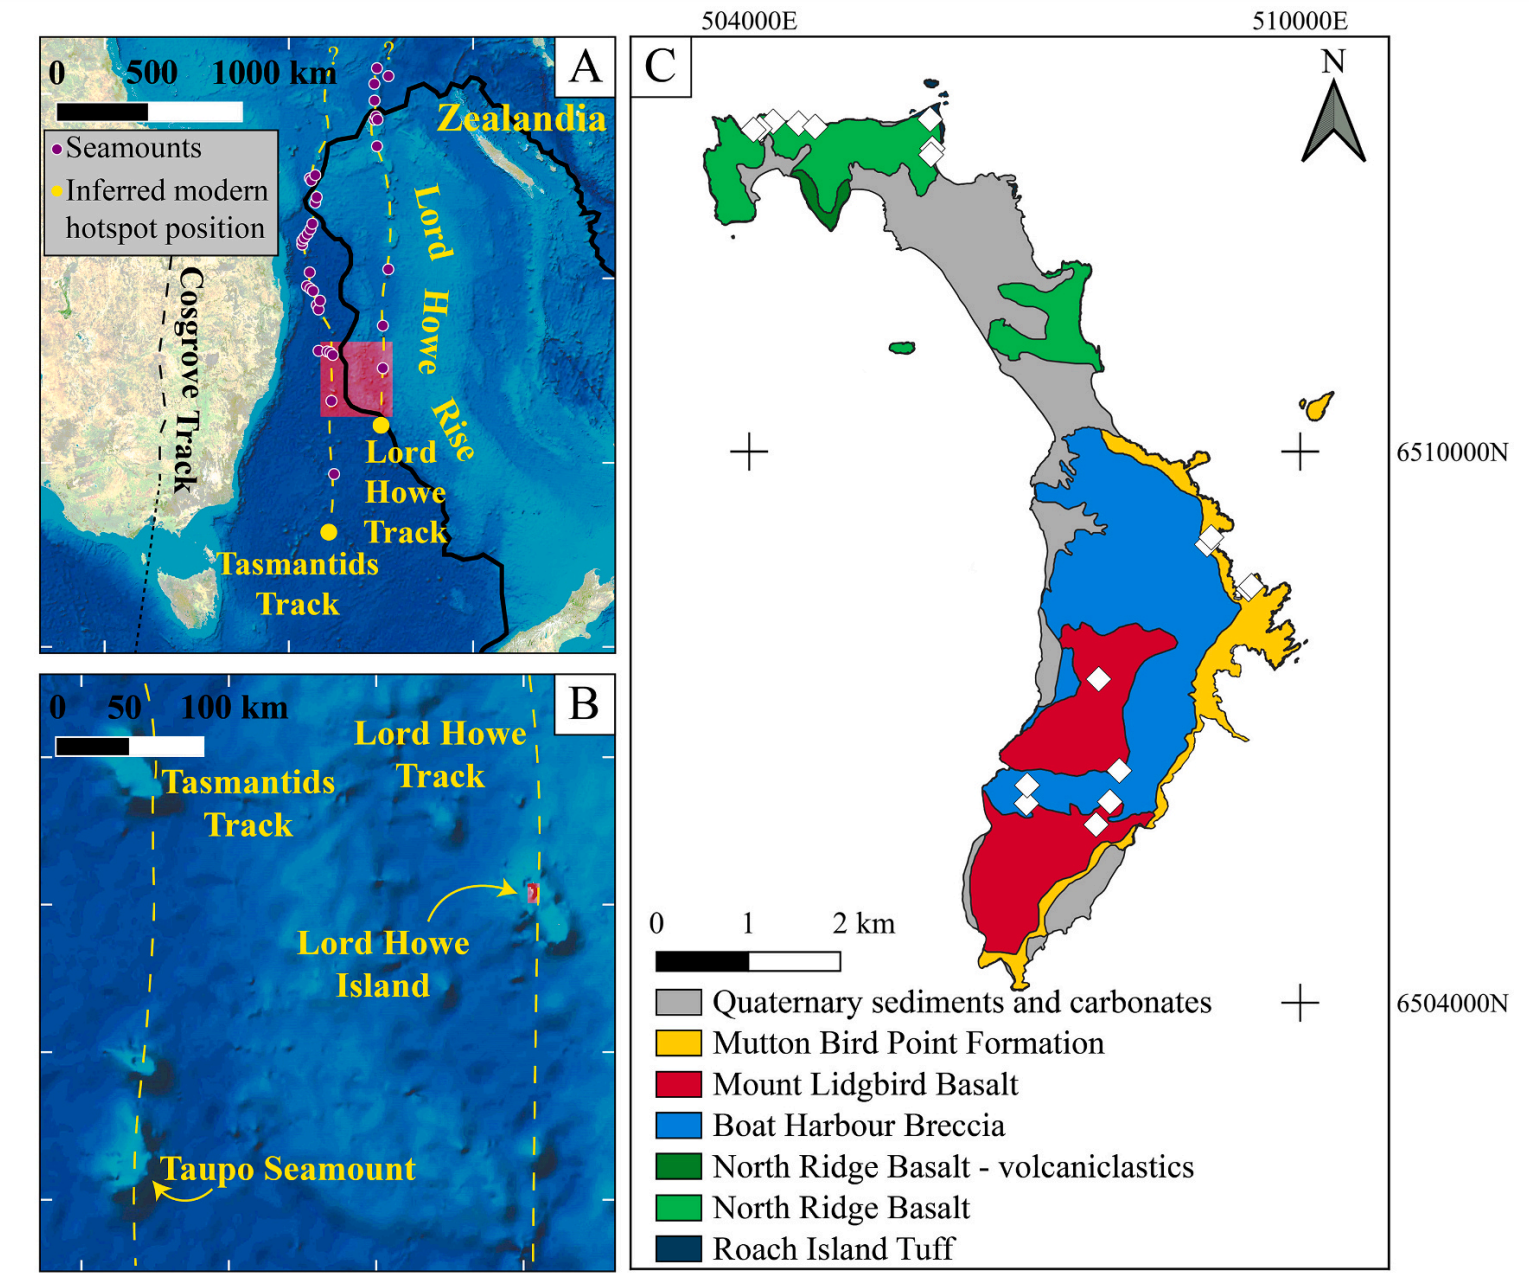
\includegraphics[scale=0.7]{img/lhi-geol1.PNG}}
\captionsetup{width=0.8\linewidth}
\captionof{figure}[Geology of Lord Howe Island]{
Source of caption\cite{lhi}:
(A) Aerial map of the eastern edge of Australia showing the parallel Cosgrove, Tasmantid and Lord Howe hotspot tracks and border of the microcontinent
Zealandia, and (B) inset showing the position of LHI. (C) Geological map of LHI, adapted from McDougall et al. (1981), with known sampling locations marked in
with white diamonds (supplementary table T1). The closely dotted black line extending to the south of Australia marks the predicted extent of the Cosgrove hotspot
track towards its present day location (Davies et al., 2015b). Units and shapefiles from the Geoscience Australia portal https://portal.ga.gov.au/}
\label{geol1}
\end{minipage}
\vskip5mm

\noindent%
\begin{minipage}{\linewidth}%
\makebox[\linewidth]{%
    \includegraphics[scale=0.12]{img/lord-howe-sea-bed1-labeled.png}}
\captionsetup{width=0.8\linewidth}
\captionof{figure}[Seabed and Proximity of Zealandia]{
The GIS layers from the government of Australia depicting the proximity
and relief of the sea floor with Australia and the geological 
region Zealandia.}
\label{geol2}
\end{minipage}
\vskip5mm



\noindent%
\begin{minipage}{\linewidth}%
\makebox[\linewidth]{%
    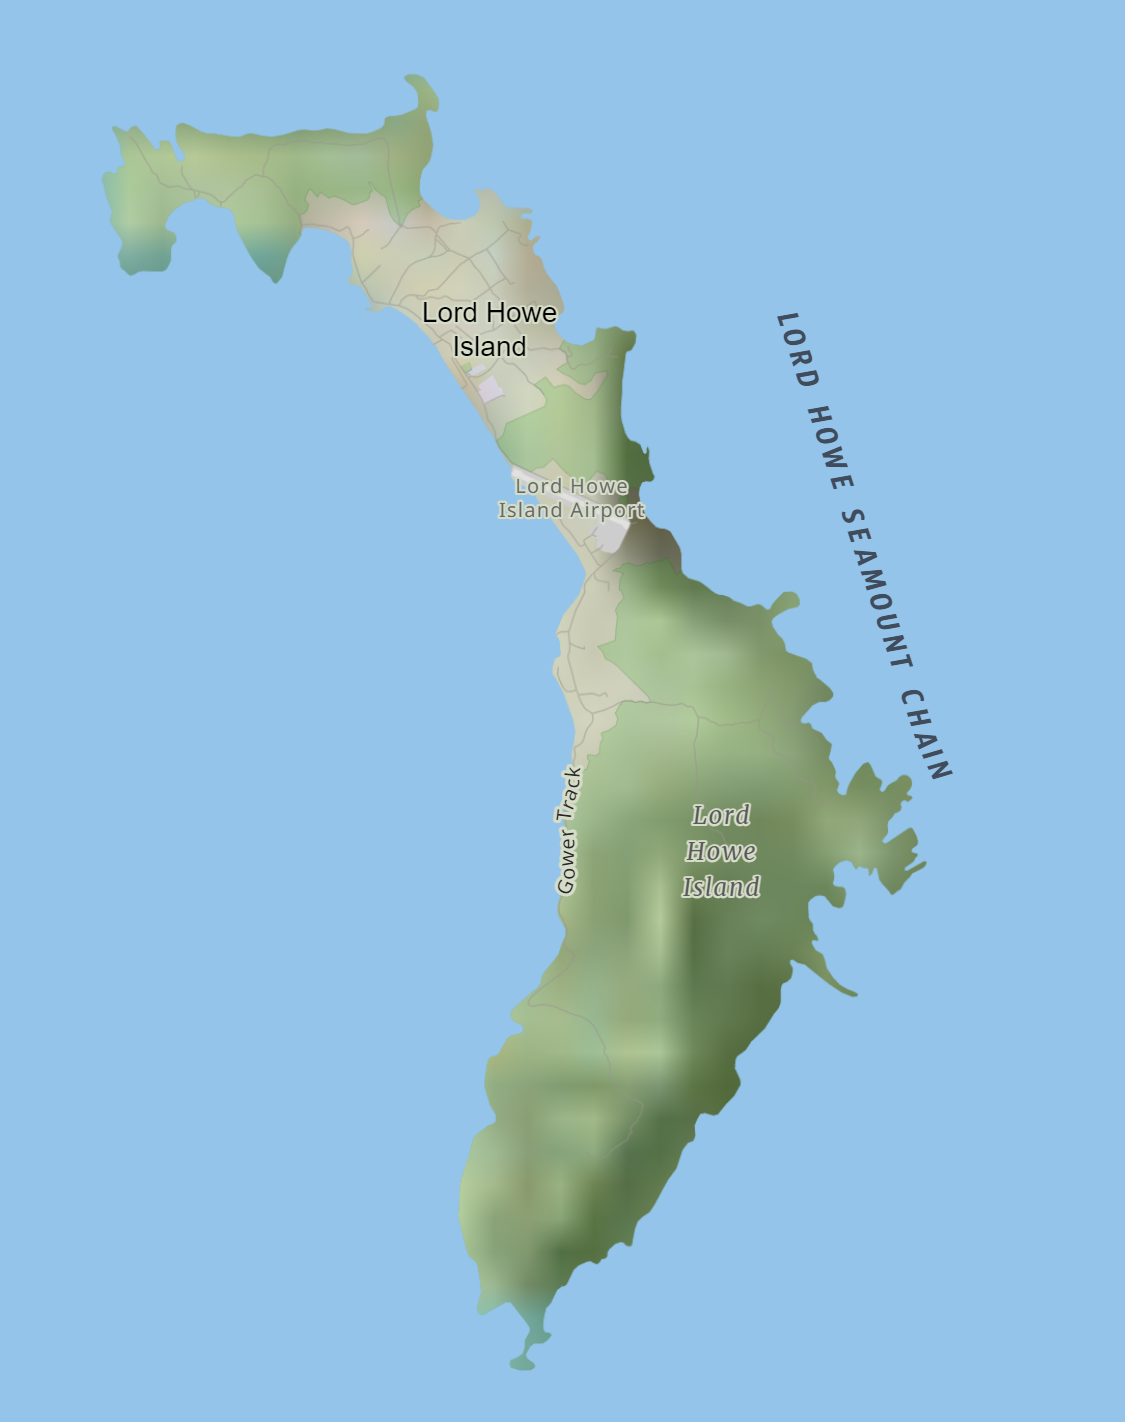
\includegraphics[scale=0.3]{img/lord-howe-island-close-cropped.png}}
\captionsetup{width=0.8\linewidth}
\captionof{figure}[Island Map Data]{ The special refuge and natural
area of the island makes up for most of the southern half and a portion
of the northwestern tip of the island.   Most of the settlement
and development on the island is in the lower half of the upper half
of the island.}
\label{geol3}
\end{minipage}
\vskip5mm

\section{Draft Announcement Letter}

When the announcement is made, this is a draft of the 
letter that will be sent out to the organizations
that track new DX'peditions:
\par
TBR -- edits to draft.
\par

\begin{Verbatim}[fontsize=\small]
To: The Daily DX, et.al.
From: Jeff Wandling W7BRS
Subject: DX'pedition to Lord Howe Island

To Whom it may concern,

This is an announcement of a DX'pedition to Lord Howe Island on 
or around July 20th through August 1st, 2024.

This is primarily a solo-expedition, but the possbility of
last minute additions to the team is not ruled out.  Contact
the Organizer (above) for details.

Synopsis:

     *  QRV on or around July 20th 2024 to Aug 1st, 2024
     *  Bands expected 80-10m (SSB, CW, and FT-8)
     *  Contest Bonus -- will be IOTA OC-004 during RSGB IOTA

The Goals:

1.   To provide a fully imersive experience with DX'pedition
     planning, deployment and execution for a semi-rare entity
     in the Pacific (Oceania) region.

2.   To experience the adventure of being on site relying on
     sound engineering judgement to setup and operate all
     common modes on as many HF bands as antenna permit (CW, SSB, Digi)
     on 80 meters through 10 meters.

3.   To engage with the local population and learn stories, history
     and document and photograph the island with an effort to bring
     back to the amateur radio community another perspective about
     this island, people and history.

4.   To lay a foundation for not only the Organizer to participate
     with future DX'peditions but also encourage and inspire those
     like the author who have dreamed for years to undertake the
     challenge of going on an adventure.

Note to Amateur Radio DX'ers:

     a)  Expect the CW to be a little slower -- 24-27 w.p.m is the goal.
     b)  Expect hours of operation to be based on limits imposed
         by weather, rest and band conditions.
     c)  Expect most QSO to be within the region of East Asia, North-
         America and Europe.  However, South American, African and
         Oceanic stations will also be worked as conditions allow.
     d)  This is a privately funded DX'pedition (no expectation of
         donations or support) -- but they will be greatly appreciated.

Lord Howe Island is currently around number 63 on ClubLog.

Expect also that Paper QSL will be offered as well as LoTW (Log Book
of the World) via OQRS.

If it was not for the support, training and advice from Northern 
California DX Foundation, Long Island DX Club, the Visalia DX 
Convention presenters and the Western Washington DX Club, this would 
not be possible.

Questions, comments and requests should be directed to the Organizer
via EMAIL.   That address is found at QRZ.com under the home-call
W7BRS


Sincerely,


Jeff Wandling, W7BRS
\end{Verbatim}

\section{Potential Request for Support}

Below is a draft of a letter that might be used if
requests for support are made with agencies, companies,
clubs or foundations.

\par
TBR -- edits to draft.
\par

\begin{Verbatim}[fontsize=\small]
To: The Daily DX, et.al.
From: Jeff Wandling W7BRS
Subject: DX'pedition to Lord Howe Island

Dear Director of Operations,

DX'peditions are the life-blood of many amateur radio operators.
Many pleasant parts of amateur radio are involved with the chasing
after good DX contacts.  The expedition that is going to happen
this July through August is one of those expeditions.

The expedtion is to Lord Howe Island, located about 700 km east of Australia.

I am a amateur radio operator who loves to chase DX and now I have a 
chance to (figureatively) put my ``feet in the sand''.  As an active
member of the Western Washington DX Club I am keeping close to those
who teach and and encourage new DX'peditions.

Your consideration of support is welcome.  I assure my effort to 
implement this DX'pedition will leverage that support in the best
way possible.

If you feel so inclined, any support you wish to offer will be greatly
appreciated.

The inspiration to do this is borne from two sources:

1.  After dreaming about doing a DX'pedition for about 14 years, I
    finally decided that unless action was taken to plan and go
    then it would never happen.  The goal in the scoping document is to 
    lay the ground work for future experiences with DX'peditions.  
    I had to start somewhere, so why not go ``full throttle'' to a 
    very exciting location.

2.  The second form of inspiration was the DX community at large.
    It began with dialog with Bob Schmieder (email) in 2011 and culminated
    with many one on one discussions Mark Aaker K6UFO, Rusty Epps W6OAT
    and Tom Berson ND2T.

    Each of them, in their own way contributed to nudging me ever closer 
    to the edge of deciding what to do and how to do it.

I look forward to hearing your signal and working your station in the
very near future from Lord Howe Island.  Wish me luck?

Sincerely,

Jeff Wandling, W7BRS
\end{Verbatim}

\newpage
\printglossary
\newpage
\bibliography{vk9l-dx-scope}{}
\printindex

\end{document}
